% Supplementary Material for paper 1037 (v25, 2026-11-09; reorganized to follow the paper), companion to main.tex, in the same official VGTC conference template.
\documentclass[preprint]{vgtc}   % single-blind: authors shown, submission ID in the page header
\usepackage[T1]{fontenc}
\usepackage{mathptmx}
\usepackage{amsmath,amssymb,amsthm}
\usepackage{booktabs,placeins,array}
\usepackage[ruled,vlined]{algorithm2e}
\SetKwInput{KwData}{Data}\SetKwInput{KwResult}{Result}
\SetKwProg{Fn}{Function}{:}{}\SetKw{KwReturn}{return}\SetKw{KwBreak}{break}
\SetKwFunction{Refine}{RefineOrder}\SetKwFunction{Barriers}{OptimalBarriers}
\SetAlFnt{\small}\SetAlCapFnt{\small\bfseries}\SetAlCapNameFnt{\small\bfseries}\DontPrintSemicolon
\newtheorem{theorem}{Theorem}\newtheorem{lemma}{Lemma}\newtheorem{proposition}{Proposition}
\renewcommand{\thesection}{S\arabic{section}}
\renewcommand{\theequation}{S\arabic{equation}}
\renewcommand{\thetheorem}{S\arabic{theorem}}
\renewcommand{\thelemma}{S\arabic{lemma}}
\renewcommand{\theproposition}{S\arabic{proposition}}
\renewcommand{\thealgocf}{S\arabic{algocf}}
\renewcommand{\thefigure}{S\arabic{figure}}
\renewcommand{\thetable}{S\arabic{table}}
% Float placement only (no change to fonts or spacing): let several figures share a page.
\renewcommand{\topfraction}{.9}\renewcommand{\dbltopfraction}{.9}\renewcommand{\textfraction}{.07}
\renewcommand{\floatpagefraction}{.75}\renewcommand{\dblfloatpagefraction}{.75}
\setcounter{topnumber}{3}\setcounter{dbltopnumber}{3}\setcounter{totalnumber}{4}
\newcommand{\dtop}{d_{\mathrm{top}}}\newcommand{\nroe}{\mathrm{NROE}}
\newcommand{\lca}{\operatorname{lca}}\newcommand{\pos}[1]{\left[#1\right]^+}
\preprinttext{Online Submission ID: 1037 --- Supplementary Material}
\onlineid{1037}
\vgtccategory{Research}
\vgtcinsertpkg

\title{Supplementary Material for AnchorMTM}

% Authors: keep identical to main.tex.
\author{%
Lele~Wang$^{1,2}$\thanks{%
Affiliations:
$^{1}$ Advanced Interactive Technology and Application Laboratory, Computer Network Information Center, Chinese Academy of Sciences, Beijing, China;
$^{2}$ University of Chinese Academy of Sciences, Beijing, China;
$^{3}$ Hangzhou Institute for Advanced Study, UCAS, Hangzhou, China.
E-mails: lelewang@cnic.cn; dongyu@cnic.cn; yxmeng@cnic.cn;
liguan@sccas.cn; wangzhe@sccas.cn; sgh@sccas.cn;
liujun@sccas.cn.
Lele Wang and Yu Dong contributed equally to this work.
Jun Liu is the corresponding author.}%
\quad
Yu~Dong$^{1,*}$%
\quad
Yuxiang~Meng$^{1,2}$%
\quad
Guan~Li$^{1,2}$%
\quad
Zhe~Wang$^{1,2}$%
\quad
Guihua~Shan$^{1,2,3}$%
\quad
Jun~Liu$^{1,2}$\thanks{Corresponding author. E-mail: liujun@sccas.cn.}
}

\hypersetup{pdftitle={Supplementary Material for AnchorMTM},pdfauthor={Lele Wang, Yu Dong, Yuxiang Meng, Guan Li, Zhe Wang, Guihua Shan, Jun Liu}}


\abstract{This document supplements the paper ``AnchorMTM: Spatially Anchored Merge Tree Maps with Position Bounds.'' It follows the order of the paper. Section~S1 fixes the notation, Section~S2 proves the bounds and the optimal barriers, and Section~S3 completes the construction. Section~S4 describes the compared methods, the data and the settings. Section~S5 adds results in the order of the evaluation, including the maps and positions of every sequence, the per-frame effect of the budget and an hourly air-pollution episode. Section~S6 lists the complete results, one table per measure, with every method in its own column.}

\begin{document}
\setcounter{section}{-1}
\firstsection{Overview}
\maketitle
The paper makes three claims: the displacement that a merge tree forces on a spatially anchored map can be bounded from the data alone; AnchorMTM attains these bounds with one merge-error budget; and existing maps pay more than the tree demands. This supplement supports each claim in the same order. It first states the conventions behind the bounds (S1) and proves them (S2). It then gives every detail of the construction that the paper summarizes (S3). Before the additional results, it describes how the compared maps were produced and how the data were prepared (S4), so that every number in S5 and S6 can be traced to a method and a configuration. The results of S5 follow the subsections of the evaluation, and S6 collects all measured values by method. Statements use the join convention; split trees are handled by negating the field, and nodes with equal merge levels form multifurcations.

\section{Notation and Error Conventions}\label{sec:interval}
This section fixes the quantities that the bounds and the measures use. For a frame, $T$ is the supplied merge tree, $\mathcal{F}$ its leaf labels, $\mathcal{D}(v)$ the descendant leaves of node $v$, and $h(v)$ its scalar level. The matrix $V$ records source LCA levels and fixed extremum values on the diagonal. References lie in $[0,L]$; widths $W_i$ are positive in the interval model, with zero widths used only for its non-strict point-model limit. The support $S_i$ contains the extremum and its leaf-arc regular samples, excluding the parent. Its centroid is their unweighted mean, and relative geometry uses Euclidean centroid distances. The frame representation is $M_t=(\pi_t,x_t,\psi_t)$.

For a fixed order $\pi$, introduce interval centers $z_i$ and anchor slack $H_i=\rho W_i/2$, with $0\le\rho\le1$. The valid-layout set $\mathcal{L}(\pi)$ consists of pairs $(x,z)$ satisfying
\begin{equation}\label{eq:layout}
\begin{aligned}
 W_i/2&\le z_i\le L-W_i/2, &0&\le x_i\le L,\\
 |x_i-z_i|&\le H_i,\\
 z_{\pi(k+1)}-z_{\pi(k)}&\ge
 (W_{\pi(k)}+W_{\pi(k+1)})/2+g,
\end{aligned}
\end{equation}
for every adjacent pair, with minimum gap $g\ge0$. A necessary capacity condition is $\sum_i W_i+(n-1)g\le L$; infeasible widths are reported rather than silently rescaled. We suppress $t$ in within-frame analysis.

Actual reference displacement is $e_i=|x_i-q_i|$, with $E_\infty=\max_i e_i/L$. An order has normalized reference-order error
\begin{equation}\label{eq:nroe}
 \nroe(\pi)=\frac{1}{2L}\max_k
 \left(\max_{j\le k}q_{\pi(j)}-q_{\pi(k)}\right).
\end{equation}
This is the smallest worst displacement divided by $L$ for a nondecreasing point placement in the specified order, ignoring widths and gaps. It is an order obstruction, not the measured displacement of the final anchors.

For $i\ne j$, the displayed merge is the maximum profile value on the interval between $x_i$ and $x_j$. Set $V_{ii}^{\psi}=\psi(x_i)$ and define
\begin{equation}\label{eq:dtop}
 \dtop(\psi,T)=\max_{i,j}|V_{ij}^{\psi}-V_{ij}|,
 \qquad\mathrm{NMLE}=\dtop/\Delta_F,
\end{equation}
where $\Delta_F>0$ is the declared scalar range, shared across the sequence. We require
\begin{equation}\label{eq:budget}
 \dtop(\psi_t,T_t)\le\eta,
 \qquad\eta=(\varepsilon_0+\varepsilon)\Delta_F.
\end{equation}
Here $\varepsilon_0$ accounts for data resolution and $\varepsilon\ge0$ is the additional analyst-selected budget. Exact topology below means zero labelled error on the declared tree; a numerical-tie allowance is accounted for through $\eta$, rather than assumed to be exactly zero on the original matrix.

If source and displayed trees are interpreted in the canonical cophenetic merge-tree representation, with fixed labels covering all their leaves and induced matrices including the diagonal values, the unnormalized discrepancy in Eq.~\ref{eq:dtop} is the labelled interleaving distance~\cite{Munch:2019:LINF,Gasparovic:2024:IID}. Under those representation conditions, $d_B\le d_I\le\dtop$ for the corresponding persistence diagrams and unlabelled trees~\cite{Gasparovic:2024:IID,Morozov:2013:IDMT}. NMLE itself is a normalized discrepancy. If rendering introduces unlabelled extrema, the anchor matrix alone does not justify this identification for the entire displayed tree.

\section{Proofs of the Bounds}\label{sec:proofs}
The paper states three bounds and the optimal barriers. This section proves them in the same order: the exact-topology bound (S2.1), the width-aware bound together with the exact evaluation of $\tau$ for a fixed order (S2.2), the bounded-topology bound (S2.3), and the optimal barriers (S2.4).

\subsection{Exact-Topology Bound}\label{sec:exact}
In a reduced tree whose proper ancestor levels strictly increase, zero labelled merge error requires every subtree's leaves to form a contiguous block. Otherwise a foreign leaf between two descendants would force a merge above that subtree's level. Equal-level events are treated as one node before imposing this requirement. For subtree $X$, let $m_X=\min_{i\in\mathcal{D}(X)}q_i$ and $M_X=\max_{i\in\mathcal{D}(X)}q_i$.

\begin{theorem}[Exact-topology order bound]\label{thm:order}
Every zero-error profile satisfies $\nroe(\pi)\ge\nu^*(T,q)$, where
\begin{equation}\label{eq:nu}
 \nu^*(T,q)=\frac{1}{2L}\max_v\max_{\substack{X,Y\in\mathrm{ch}(v)\\X\ne Y}}
 \pos{\min(M_X-m_Y,M_Y-m_X)}.
\end{equation}
Recursively ordering each node's children by reference-hull midpoint $(m_X+M_X)/2$ attains this bound for the point-order objective, in $O(n\log n)$ time.
\end{theorem}
\begin{proof}[Proof sketch]
If block $X$ precedes block $Y$, an inversion from $M_X$ to $m_Y$ requires worst point displacement at least $[M_X-m_Y]^+/2$. Reversing the blocks gives $[M_Y-m_X]^+/2$. Every legal order must choose one orientation. Midpoint order chooses the less costly one since $m_X+M_X\le m_Y+M_Y$ is equivalent to $M_X-m_Y\le M_Y-m_X$. Every inverted leaf pair belongs to different child blocks at its lowest common ancestor, so the largest of these sibling costs also bounds all inversions from above in the midpoint order.
\end{proof}
The certificate depends only on the source tree and references, not on an observed layout or optimizer. It applies to any exact profile, including outputs of TMTM and ST-MTM with the same feature tree. Attainment refers to Eq.~\ref{eq:nroe}: it does not assert that a finite-width layout or its final quadratic placement attains $L\nu^*$.

\subsection{Width-Aware Bounds and Fixed-Order Evaluation}\label{sec:width}
For nonoverlapping finite intervals, the fixed-order minimax cost is
\begin{equation}\label{eq:tau}
 \tau(\pi)=\min_{(x,z)\in\mathcal{L}(\pi)}\|x-q\|_\infty.
\end{equation}
The canvas is compact, so the minimum is attained when the layout set is nonempty. Widths, gaps, and canvas ends may force displacement even when the reference order is feasible in the point model. Set
\begin{equation}
 \ell_i=q_i-W_i/2-H_i,\quad h_i=q_i+W_i/2+H_i,
 \quad s_i=W_i+g.
\end{equation}
For a nonempty leaf set $S$, define packing summaries
\begin{equation}\label{eq:AB}
\begin{aligned}
 A(S)&=\max_{\alpha\in\{\ell_i:i\in S\}}
 \left(\alpha+\sum_{\substack{i\in S\\\ell_i\ge\alpha}}s_i\right),\\
 B(S)&=\max_{\zeta\in\{h_i:i\in S\}}
 \left(\sum_{\substack{i\in S\\h_i\le\zeta}}s_i-\zeta\right).
\end{aligned}
\end{equation}
Here $A(X)$ abbreviates $A(\mathcal{D}(X))$, and likewise for $B$.

\begin{theorem}[Width-aware bound]\label{thm:width}
If all leaves of $X$ precede all leaves of $Y$, every valid placement has worst displacement at least $(A(X)+B(Y)-g)/2$. Consequently every exact-topology interval layout satisfies $\tau(\pi)\ge\mathcal{B}_w(T,q,W)$, where
\begin{equation}\label{eq:widthbound}
\begin{aligned}
\mathcal{B}_w&=\max\{0,B(\mathcal{F})-g,A(\mathcal{F})-g-L,K_w\},\\
K_w&=\max_v\max_{X\ne Y\in\mathrm{ch}(v)}
 \frac{\min\{A(X)+B(Y),A(Y)+B(X)\}-g}{2}.
\end{aligned}
\end{equation}
\end{theorem}
\begin{equation}\label{eq:pack}
 z_b-z_a\ge\sum_{k\in S}s_k-g-W_a/2-W_b/2.
\end{equation}
Here $a,b$ enclose every selected interval in $S$; other intervals only increase the required span.
\begin{proof}
(i) Take $S_X\subseteq X$, $S_Y\subseteq Y$, let $a$ be the first leaf of $S_X$ and $b$ the last leaf of $S_Y$ in the order. All of $S=S_X\cup S_Y$ lies between them, so by (\ref{eq:pack}) and the anchor slack, $x_b-x_a\ge\sum_S s_k-g-W_a/2-W_b/2-H_a-H_b$. Since $\tau\ge q_a-x_a$ and $\tau\ge x_b-q_b$,
\begin{align*}
\tau&\ge\tfrac12\big[(q_a-x_a)+(x_b-q_b)\big]\ge\tfrac12\Big[\ell_a-h_b+\sum_{k\in S}s_k-g\Big]\\
&\ge\tfrac12\Big[\min_{S_X}\ell+\sum_{S_X}s_k+\sum_{S_Y}s_k-\max_{S_Y}h-g\Big].
\end{align*}
For $S_X=\{k\in X:\ell_k\ge\alpha\}$ the first two terms are at least $\alpha+\sum_{k\in X,\ell_k\ge\alpha}s_k$; for $S_Y=\{k\in Y:h_k\le\zeta\}$ the last ones are at least $\sum_{k\in Y,h_k\le\zeta}s_k-\zeta$. The two choices are independent, so maximizing each gives $A(X)$ and $B(Y)$. Each maximum is over upper (resp.\ lower) sets of one sorted list and is computed by one sort and a prefix sum.
(ii) Let $b$ be the last leaf of a set $S$. The intervals of $S$ lie in $[0,z_b+W_b/2]$, so $z_b\ge\sum_S s_k-g-W_b/2$, $x_b\ge z_b-H_b$ and $\tau\ge x_b-q_b\ge\sum_S s_k-g-h_b\ge\sum_S s_k-g-\max_S h$. Lower sets of $h$ give $B(\mathrm{all})-g$. The right end is symmetric with the first leaf of $S$ and gives $A(\mathrm{all})-g-L$.
(iii) Then $\ell=h=q$, $s=0$, $A(X)=M_X$, $B(Y)=-m_Y$, and $\min(A(X)+B(Y),A(Y)+B(X))/2=\min(M_X-m_Y,M_Y-m_X)/2$, which is $L$ times the term of $\nu^*$.
\end{proof}
The summaries are evaluated by sorting and cumulative sums. With zero widths and gaps, $A(X)=M_X$ and $B(Y)=-m_Y$, and the bound reduces to $L\nu^*$. For finite widths, Eq.~\ref{eq:widthbound} is a universal lower bound, not a formula for the globally optimal order or a promise of attainment.

For a specified order, the implementation also evaluates $\tau$ exactly. Index quantities in order as $w_k=W_{\pi(k)}$, $Q_k=q_{\pi(k)}$, and $H_k=\rho w_k/2$, and define packed left and right distances
\[
 D_k=\sum_{j<k}w_j+w_k/2+(k-1)g,\quad
 R_k=\sum_{j>k}w_j+w_k/2+(n-k)g.
\]
The implemented interval-cost expression is
\begin{equation}\label{eq:fixedtau}
\begin{split}
\tau(\pi)=\max\bigg\{&0,\ \max_k(D_k-Q_k-H_k),\\
 &\max_k(Q_k-H_k-L+R_k),\\
 &\max_{j<k}\frac{Q_j-Q_k+D_k-D_j-H_j-H_k}{2}\bigg\}.
\end{split}
\end{equation}
These are boundary and pairwise packing requirements for the fixed-order interval problem. This exact subproblem cost, also available through a minimax linear program, is distinct from the tree-wide lower bound in Theorem~\ref{thm:width}.

\paragraph{Why the fixed-order evaluation is exact.}
Let $P=\sum_k w_k+(n-1)g\le L$ and $s_0=L-P$. Write the centers as $z_{\pi(k)}=D_k+y_k$. The interval constraints are equivalent to $0\le y_1\le\cdots\le y_n\le s_0$. An anchor within $H_k$ of its center and within distance $t$ of $Q_k$ exists exactly when
\[
 Q_k-D_k-H_k-t\le y_k\le Q_k-D_k+H_k+t.
\]
After intersecting these bounds with $[0,s_0]$, a nondecreasing sequence exists if and only if every prefix maximum of the lower bounds does not exceed the corresponding upper bound. Expanding this condition gives precisely the left-boundary, right-boundary and pairwise terms in Eq.~\ref{eq:fixedtau}, together with $t\ge0$. Conversely, choosing prefix maxima supplies feasible centers at the largest of those terms, and each anchor can be chosen in the intersection of its center-slack interval and $[Q_k-t,Q_k+t]$. Thus the expression is attained. This explains the implemented fixed-order evaluation; it does not optimize the leaf permutation.


\subsection{Chain-Aware Separation and Bounds}\label{sec:chain}
Allowing $\eta>0$ relaxes some displayed merge relationships, but does not eliminate all separation constraints. We use $\eta$ in scalar units throughout this analysis to avoid confusing it with the normalized budget $\varepsilon$.

\begin{lemma}[Separation]\label{lem:sep}
Let $i,j\in\mathcal{D}(u)$ and let leaf $k$ lie strictly between their anchors. If $\dtop\le\eta$, then $V_{ik}\le h(u)+2\eta$.
\end{lemma}
\begin{proof}
The interval from $i$ to $k$ is contained in that from $i$ to $j$, so
$V_{ik}-\eta\le V_{ik}^{\psi}\le V_{ij}^{\psi}
\le V_{ij}+\eta\le h(u)+\eta$.
\end{proof}

Let $A_\eta(u)$ be the highest ancestor of $u$ with level at most $h(u)+2\eta$. This ancestor is determined by the total level difference from $u$, not by testing each parent gap independently.
\begin{theorem}[Chain-aware separation and bounds]\label{thm:chain}
No leaf outside $\mathcal{D}(A_\eta(u))$ can occur between two leaves of $u$ in a profile with $\dtop\le\eta$. Further, if
\begin{equation}\label{eq:chainpair}
\begin{aligned}
 \mathcal{D}(w)\cap\mathcal{D}(A_\eta(u))&=\varnothing,\\
 \mathcal{D}(u)\cap\mathcal{D}(A_\eta(w))&=\varnothing,
\end{aligned}
\end{equation}
then all leaves of $u$ precede all leaves of $w$, or conversely. For all such separated pairs $(X,Y)$, including $(u,\{k\})$ with $k\notin\mathcal{D}(A_\eta(u))$, valid lower bounds are
\begin{equation}\label{eq:chainbounds}
\begin{aligned}
 \nroe(\pi)&\ge\frac{1}{2L}\max_{(X,Y)}
 \pos{\min(M_X-m_Y,M_Y-m_X)},\\
 \tau(\pi)&\ge\max_{(X,Y)}
 \frac{\min\{A(X)+B(Y),A(Y)+B(X)\}-g}{2}.
\end{aligned}
\end{equation}
The order-independent canvas terms and zero remain part of the width-aware bound.
\end{theorem}
\begin{proof}[Proof sketch]
A leaf outside $A_\eta(u)$ merges with each descendant of $u$ above $h(u)+2\eta$, so Lemma~\ref{lem:sep} excludes it from the span of $u$. Under Eq.~\ref{eq:chainpair}, neither leaf set can interleave the other. If one set occupied both sides of the other, the latter would lie between two of its leaves, also contradicting separation. The two possible block orientations give Eq.~\ref{eq:chainbounds} by the same inversion and packing arguments as before.
\end{proof}
A coarser certificate flattens internal nodes whose parent gaps are at most $2\eta$ and applies the exact-topology bounds to the remaining hierarchy. The chain certificate includes the separated pairs used by that bound and also accounts for accumulated gaps along ancestor chains. These certificates express necessary conditions for every budget-feasible layout; they do not construct a feasible order by themselves.

The relaxation concerns merge levels in the displayed profile. The input field, its extracted extrema, and supplied feature identities remain the reference data. The budget is an upper allowance, while measured NMLE records the amount actually used. Increasing it can enlarge the feasible set but does not guarantee smaller displacement for every feature, nor does it establish that a heuristic search returns a better layout at every budget.


For clarity, $C_\eta(T,q)$ is the right-hand side of the first inequality in Eq.~\ref{eq:chainbounds}. Let $K_{w,\eta}$ be the right-hand side of its second inequality. The full width-aware chain certificate is
\begin{equation}\label{eq:chaincertificate}
 C_{w,\eta}(T,q,W)=\max\{0,K_{w,\eta},B(\mathcal{F})-g,A(\mathcal{F})-g-L\}.
\end{equation}
Thus both chain certificates include all eligible node--leaf pairs and mutually excluded node--node pairs; the width-aware one also includes the canvas-end terms. Singleton sets use $A(\{k\})=\ell_k+s_k$ and $B(\{k\})=s_k-h_k$. The ancestor test measures the full height difference, not each parent gap independently. All budget calculations use absolute scalar units $\eta$.
\subsection{Optimal Merge Barriers}\label{sec:barriers}
Changing the leaf order changes which feature pairs span each inter-feature gap. Simply retaining the original LCA value of each adjacent pair need not minimize the resulting merge error. Let $b_k$ be the barrier between leaves $\pi(k)$ and $\pi(k+1)$. The merge level displayed between positions $i<j$ is
\begin{equation}\label{eq:maxbarrier}
 V_{\pi(i)\pi(j)}^{\psi}=\max_{i\le k<j}b_k.
\end{equation}
For fixed extremum values $v_i=V_{ii}$, define
\begin{equation}
 C_k=\min_{i\le k<j}V_{\pi(i)\pi(j)},\quad
 F_k=\max(v_{\pi(k)},v_{\pi(k+1)}).
\end{equation}
\begin{proposition}[Optimal barriers]\label{prop:barriers}
The minimum labelled merge error for the fixed order and extremum values in the continuous non-strict model is
\begin{equation}\label{eq:delta}
\begin{split}
\delta^*(\pi)=\max\bigg\{&0,\ \max_k(F_k-C_k),\\
 &\frac12\max_{i<j}\left(V_{\pi(i)\pi(j)}-
                         \max_{i\le k<j}C_k\right)\bigg\},
\end{split}
\end{equation}
and $b_k=C_k+\delta^*(\pi)$ attains it.
\end{proposition}
\begin{proof}
The displayed merge of the $i$th and $j$th leaf is $\max_{i\le k<j}b_k$, and each barrier must be at least $F_k$ to keep both basins. An error $\delta$ requires $b_k\le V_{\pi(i)\pi(j)}+\delta$ for every pair spanning $k$, i.e., $b_k\le C_k+\delta$; it also requires $\max_{i\le k<j}b_k\ge V_{\pi(i)\pi(j)}-\delta$ and $b_k\ge F_k$. The largest admissible barriers $b_k=C_k+\delta$ satisfy all constraints exactly when $\delta$ is at least each term of $\delta^*$; smaller barriers only lower the maxima. Hence $\delta^*$ is optimal and attained.
\end{proof}
For fewer than two leaves the barrier list is empty and $\delta^*=0$. For an exact-tree order, $\delta^*=0$ and the barriers agree with the relevant adjacent LCA levels. For a conflicting order, the minimax solution balances raised and lowered displayed merges. This exact calculation provides the topology oracle in Eq.~\ref{eq:budget}; it does not establish global optimality of the order search. The implemented direct evaluation costs $O(n^3)$ per order. The proposition permits equality at a leaf value. A raster implementation requiring strict extrema may add a small clearance, which must be counted separately in the measured rendered error.

\begin{algorithm}[tp]
\caption{Optimal Merge Barriers for a Fixed Leaf Order}\label{alg:barriers}
\KwData{Order $\pi$ and source merge matrix $V$, including original extremum values $V_{ii}$.}
\KwResult{Minimum continuous labelled merge error $\delta^*(\pi)$ and optimal barriers $b$.}
\Fn{\Barriers{$\pi,V$}}{
 $n\leftarrow|\pi|$; $\delta\leftarrow0$\;
 \If{$n<2$}{\KwReturn{$(0,\varnothing)$}\;}
 \For{$k\leftarrow1$ \KwTo $n-1$}{
  $C_k\leftarrow\min_{1\le i\le k<j\le n}V_{\pi(i)\pi(j)}$\;
  $F_k\leftarrow\max\{V_{\pi(k)\pi(k)},V_{\pi(k+1)\pi(k+1)}\}$\;
  $\delta\leftarrow\max\{\delta,F_k-C_k\}$\;
 }
 \For{each pair $1\le i<j\le n$}{
  $\delta\leftarrow\max\{\delta,\tfrac12(V_{\pi(i)\pi(j)}-\max_{i\le k<j}C_k)\}$\;
 }
 \For{$k\leftarrow1$ \KwTo $n-1$}{
  $b_k\leftarrow C_k+\delta$\;
 }
 \KwReturn{$(\delta,b)$}\;
}
\end{algorithm}

\FloatBarrier
\section{Construction Details}\label{sec:construction}
AnchorMTM computes a map from the field sequence and the budget $\varepsilon$ alone. This section completes the three stages of the paper: the overall algorithm (S3.1), the candidate leaf orders (S3.2), the placement program (S3.3), the profile reconstruction and its checks (S3.4), and the conventions of the implementation (S3.5).

\subsection{Complete Algorithm and Schematics}\label{sec:supp_construction}
Algorithm~\ref{alg:construction} lists the complete construction of the paper, separating the discrete order selection from fixed-order placement. Figure~\ref{fig:direction-open} illustrates the motion-derived reference, and Fig.~\ref{fig:selective_relaxation} shows how a selective flattening admits the order $A,C,D,B$ while keeping the $C,D$ grouping; such a proposal is still evaluated against the original merge matrix and the budget (Section~\ref{sec:search}).

\begin{algorithm}[htbp]
\caption{Single-Control AnchorMTM}\label{alg:construction}
\KwData{2D/3D field sequence and grid; $\varepsilon\ge0$; fixed configuration $\Theta_0$.}
\KwResult{Temporal map $I^\varepsilon$, error records, or a failure report.}
Extract augmented trees, leaf supports and extrema; match supports and assign Track IDs\;
Estimate one direction and fixed references $q_t$; reuse this preprocessing across budgets\;
$\eta\leftarrow(\varepsilon_0+\varepsilon)\Delta_F$\;
\For{each time step $t$ in temporal order}{
 Report and stop if widths and gaps exceed the fixed canvas\;
 $\mathcal{C}_t\leftarrow\operatorname{GenerateAndRefine}(T_t,q_t,W_t,V_t,\eta)$; retain strict-topology candidates\;
 Evaluate $\tau(\pi)$, $\nroe(\pi)$ and $\delta^*(\pi)$ for candidates\;
 $\mathcal{F}_t\leftarrow\{\pi\in\mathcal{C}_t:\delta^*(\pi)\le\eta\}$\;
 \lIf{$\mathcal{F}_t=\varnothing$}{report no feasible candidate and stop}
 Select $\pi_t^\varepsilon$ from $\mathcal{F}_t$ by $(\tau,\nroe)$\;
 Compute optimal merge barriers for $\pi_t^\varepsilon$\;
 Solve the four-term QP only for $\pi_t^\varepsilon$, with cap $\tau(\pi_t^\varepsilon)+\beta_0$ and valid matched history\;
 Reconstruct the profile by leaf/LCA filling and barrier correction\;
 Record candidate counts, continuous and rendered errors, motion and failures; append profile to $I^\varepsilon$\;
}
\KwReturn{$I^\varepsilon$ and diagnostic records}\;
\end{algorithm}
\begin{figure}[t]
\centering
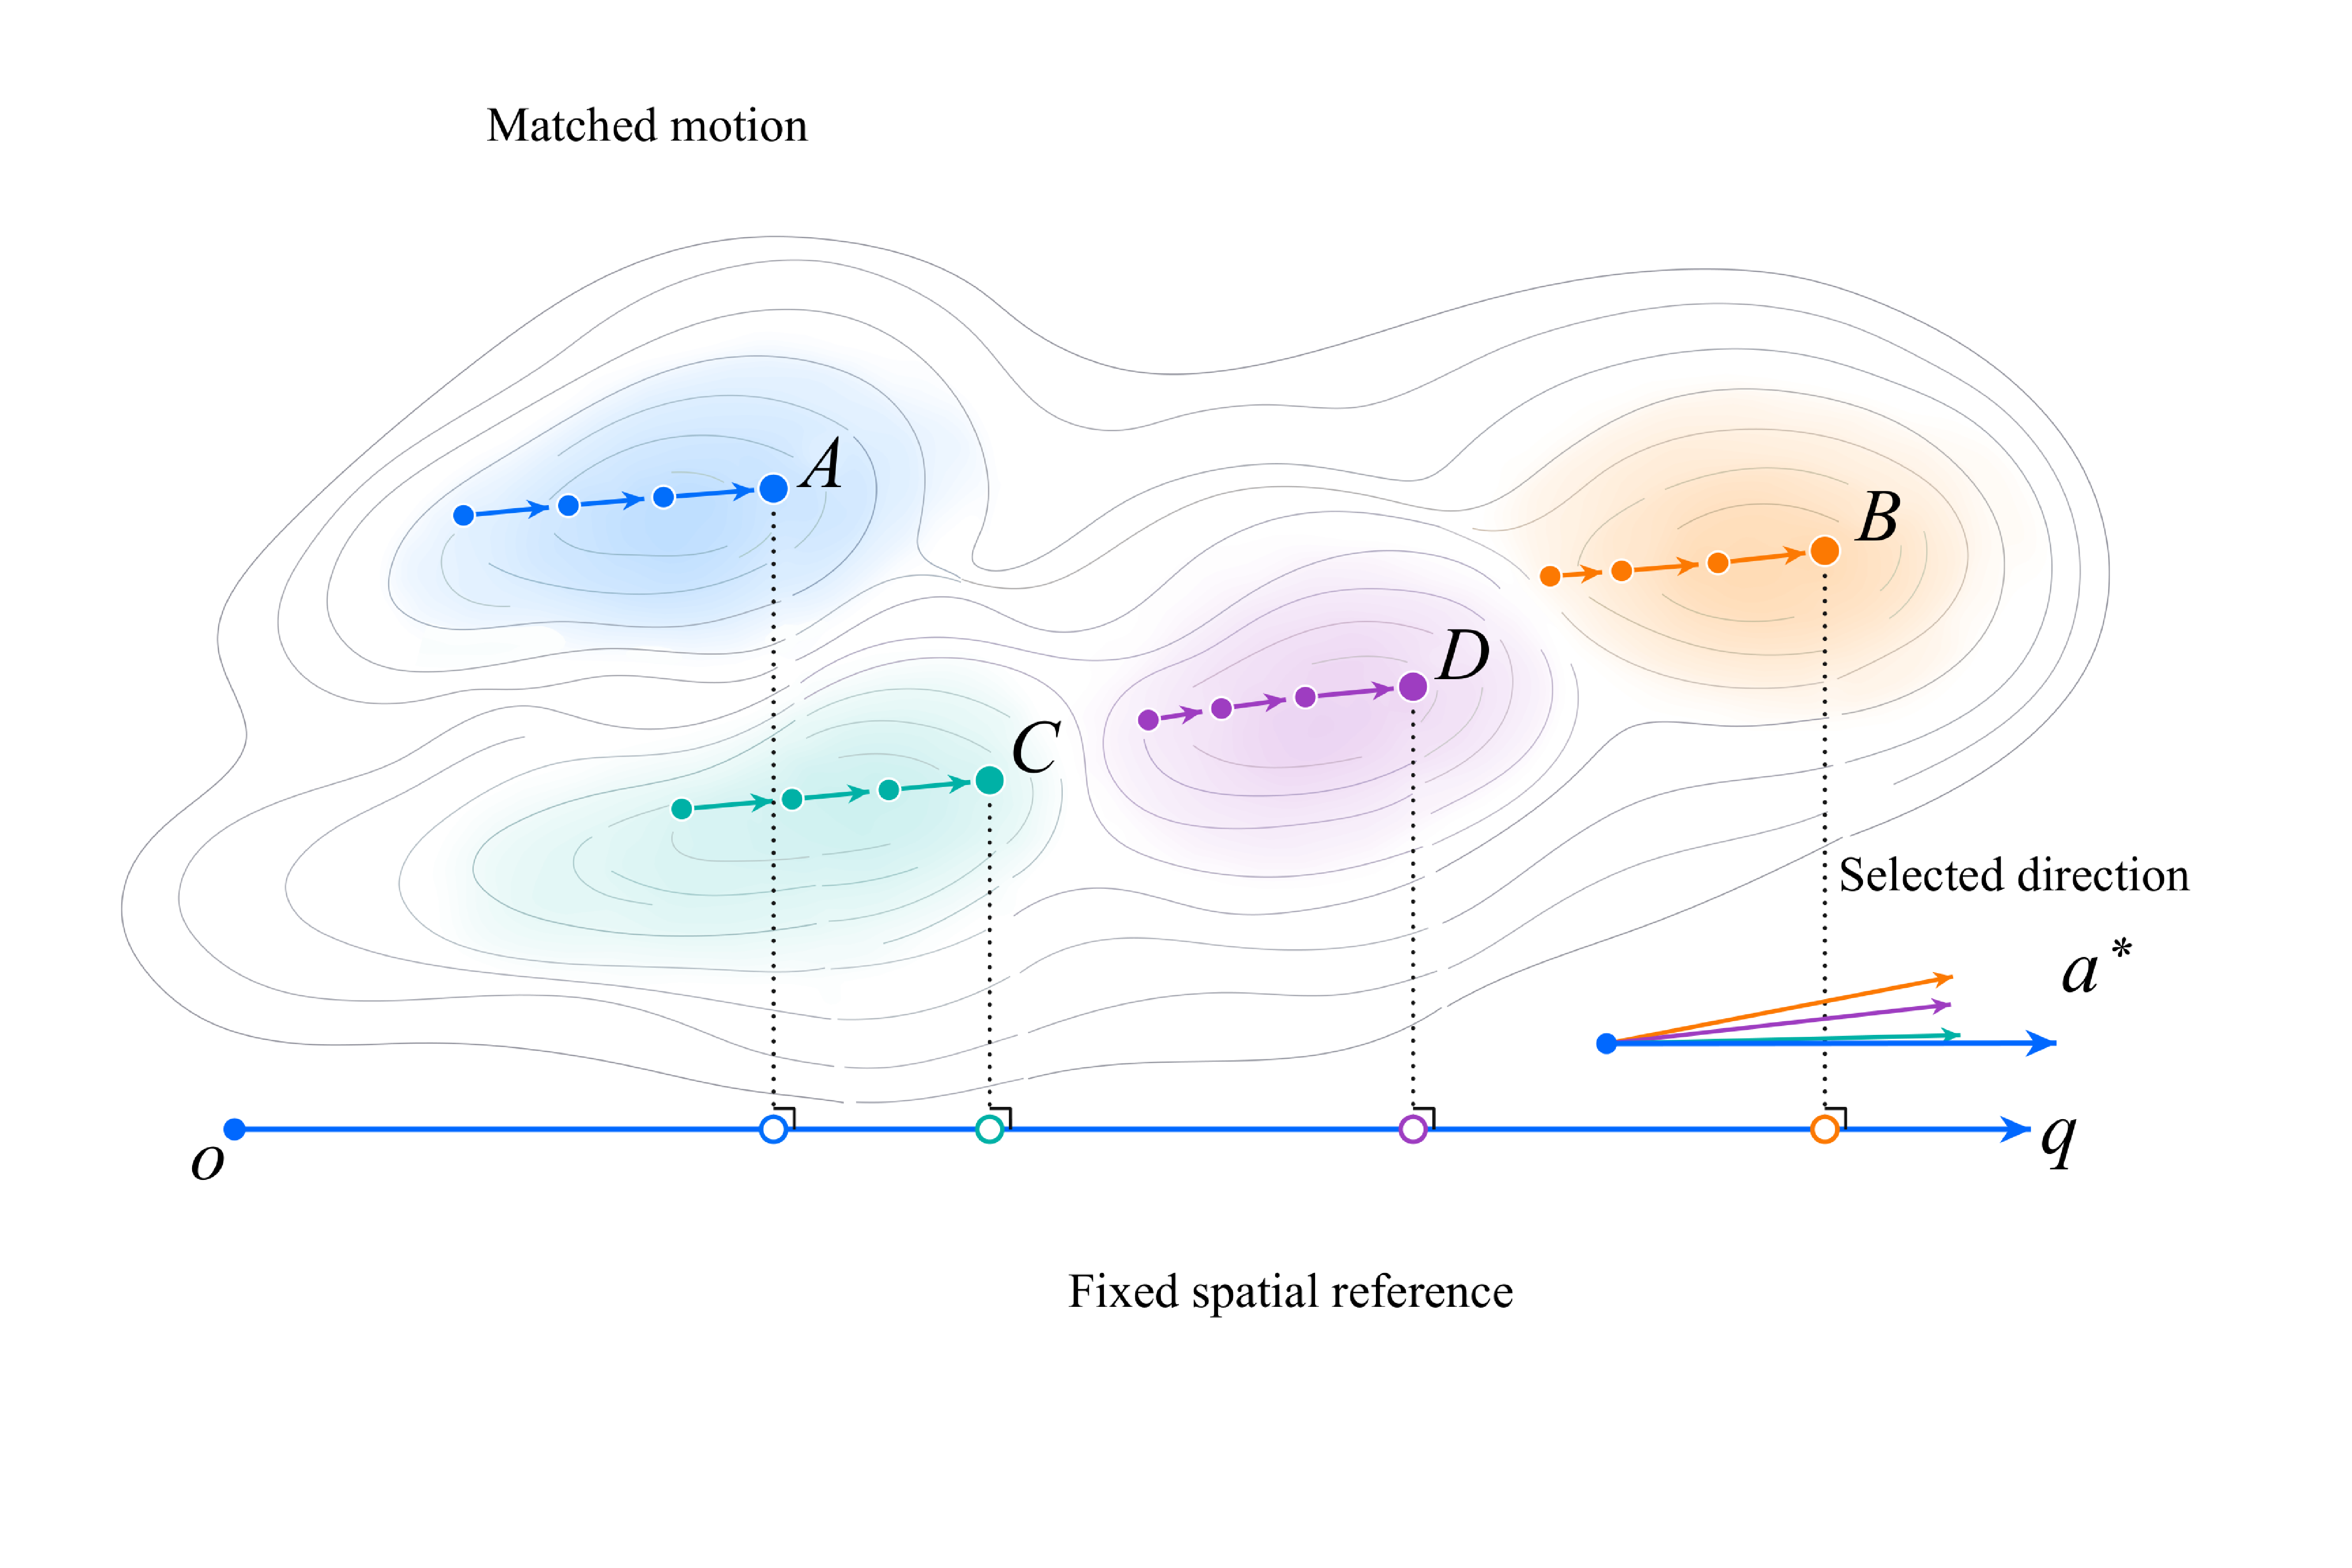
\includegraphics[width=0.85\columnwidth]{figures/anchor_direction_open.pdf}
\caption{Motion-derived spatial reference. Matched extremum displacements define one direction $a^*$ for the sequence; extrema project onto the parallel reference axis $q$ from a common origin $o$. Tracks, contours and projection positions are schematic.}
\label{fig:direction-open}
\end{figure}
\begin{figure}[t]
\centering
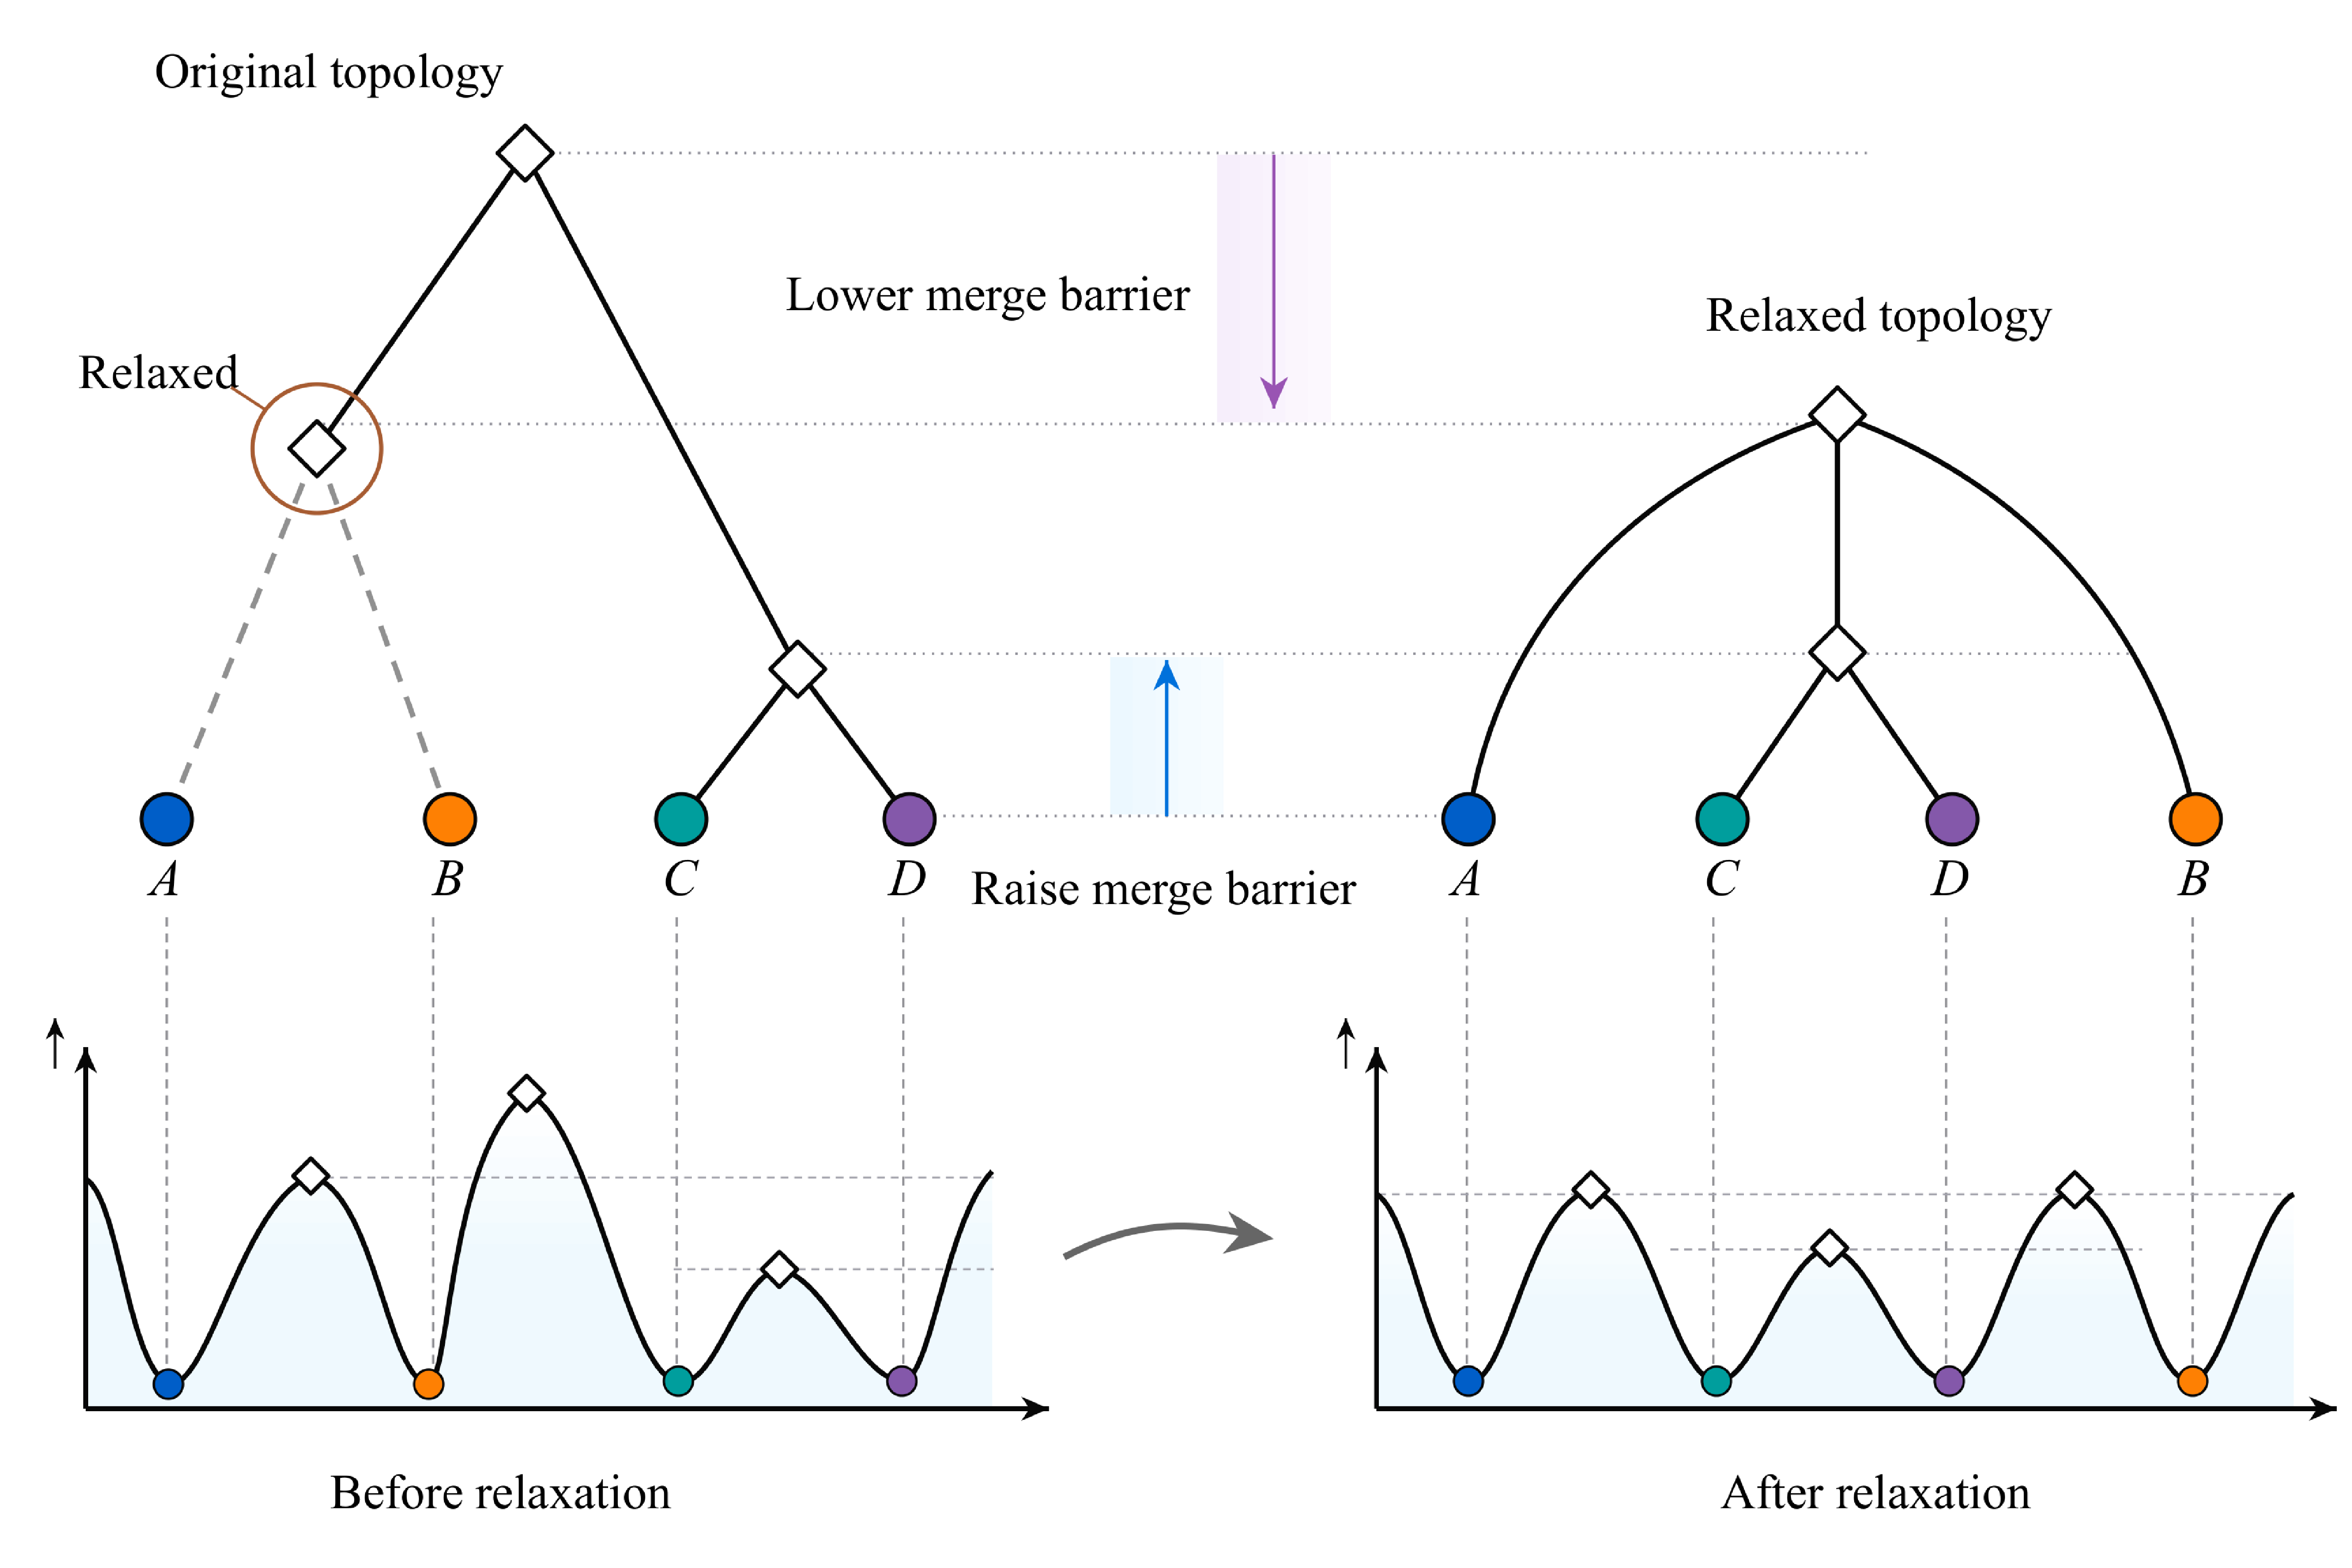
\includegraphics[width=\columnwidth]{figures/anchor_relaxation_open.pdf}
\caption{Selective relaxation releases the $A,B$ block constraint and admits order $A,C,D,B$ while retaining the $C,D$ grouping. The accompanying profiles illustrate changed merge barriers; source-level guides show the hierarchy changes. Heights are schematic, and candidate orders still require evaluation against the original merge matrix.}
\label{fig:selective_relaxation}
\end{figure}

\subsection{Candidate Generation and Width-Aware Refinement}\label{sec:search}
The following details specify the AnchorMTM heuristic over a restricted family of candidate orders. The source matrix is used by every merge-budget check. Midpoint initialization, threshold and conflict-driven candidates, and the retained point order are the same as in the main-paper algorithm.

\emph{Candidate structures.} The helper returns the exact tree, threshold flattenings for distinct internal parent gaps up to $2\eta$, and the retained conflict-driven selective flattening. Selective generation starts from the exact tree and considers releasing one or both internal blocks of the sibling pair with the largest order obstruction. Trials respect accumulated ancestor gaps, pass Eq.~\ref{eq:budget}, and are compared by NROE, merge cost, and number of newly released nodes. Non-worsening NROE steps may continue the search; the best strictly improving state is retained. The point candidate $\pi_p$ is the best feasible threshold midpoint order by NROE, replaced by the selective order only if it improves NROE. This is a finite heuristic candidate family, not enumeration of every permutation.

\emph{Refinement and selection.} In the refinement, $\sigma$ is the sum of squared positive boundary and pair terms in Eq.~\ref{eq:fixedtau}. Initial structures are ranked by $(\tau,\sigma,\text{number released})$. A refinement uses every insertion position for nodes with at most eight children and positions within distance three otherwise. A move must improve $(\tau,\sigma)$ lexicographically and pass the exact topology check; comparisons use the implementation's numerical tolerances. Retaining $\pi_p$ ensures that the final $(\tau,\nroe)$ selection cannot worsen its fixed-order displacement. Exact midpoint optimality, exact evaluation of $\tau$, and heuristic leaf-order search are separate guarantees. Exhaustive enumeration certifies a global order optimum only when all permutations are covered.

The algorithm assumes the widths fit the canvas under Eq.~\ref{eq:layout}. The exact-tree candidate supplies a feasible continuous topology order; width-capacity failure and insufficient raster resolution are reported by the corresponding routines. For $\eta=0$, the certificate helper uses the exact-topology bounds; for $\eta>0$, it evaluates the coarse and chain-aware certificates and retains the stronger applicable bound. These values are reported as benchmarks of unavoidable error. Candidate refinement and final selection use exact fixed-order costs; the certificates are not used as search-pruning thresholds.


\begin{algorithm}[htbp]
\caption{Width-Aware Refinement of One Candidate Structure}\label{alg:refine}
\KwData{Initialized structure $S$ and order $\pi$; references, widths, source merge matrix and scalar budget.}
\KwResult{A budget-feasible refined order.}
\Fn{\Refine{$S,\pi,q,W,V,\eta$}}{
 \For{at most eight passes}{
  \For{each internal node of $S$ in traversal order}{
   Enumerate single-child-block insertions\;
   Find the first improving, budget-feasible move in $(\tau,\sigma)$ order\;
   Apply the move if one exists\;
  }
  \If{no move was accepted}{\KwBreak\;}
 }
 \KwReturn{$\pi$}\;
}
\end{algorithm}

\subsection{Complete Placement Model}\label{sec:placement}
After choosing $\pi_t$, we optimize anchors and interval centers over $\mathcal{L}(\pi_t)$. Let $P_t=\{(i,j):i\text{ precedes }j\text{ in }\pi_t\}$, and let $\gamma_i^t\in[0,1]$ be an optional confidence for a supplied temporal match. Default confidence is one. The reference-aligned target is
\[
 y_i^t=x_{\mu_t(i)}^{t-1}+\Delta q_i^t,\qquad i\in\mathcal{C}_t.
\]
The implemented normalized objective has four terms:
\begin{equation}\label{eq:qpterms}
\begin{aligned}
 E_R&=\frac1{n_t}\sum_i(x_i^t-q_i^t)^2,\\
 E_G&=\frac1{\max(1,|P_t|)}\sum_{(i,j)\in P_t}
                 (x_j^t-x_i^t-d_{ij}^t)^2,\\
 E_M&=\frac1{\max(1,|\mathcal{C}_t|)}\sum_{i\in\mathcal{C}_t}
                     \gamma_i^t(x_i^t-y_i^t)^2,\\
 E_C&=\frac1{n_t}\sum_i(x_i^t-z_i^t)^2.
\end{aligned}
\end{equation}
Fixed order turns signed separations into linear expressions, so this is a convex quadratic objective. The cap enforces position fidelity while geometry and temporal terms choose among acceptable placements:
\begin{equation}\label{eq:qp}
\begin{aligned}
 \min_{x_t,z_t}\quad&\lambda_R E_R+\lambda_G E_G+
                       \lambda_M E_M+\lambda_C E_C\\
 \text{subject to}\quad&(x_t,z_t)\in\mathcal{L}(\pi_t),\\
 &\|x_t-q_t\|_\infty\le\tau(\pi_t)+\beta,\qquad\beta\ge0.
\end{aligned}
\end{equation}
In the formulas below, $\beta$ denotes the fixed $\beta_0$. The parameter-class defaults are $(\lambda_R,\lambda_G,\lambda_M,\lambda_C)=(4,1,0.5,0.1)$, $\rho=0.5$, and $\beta=1$ in canvas units. Canvas extent, gap, and width scale are input-dependent quantities in those same units; their class defaults are $120$, $0.5$, and $0.06$, respectively. They are not universal physical settings, and an evaluation must report any overrides. Equation~\ref{eq:qp} uses term means, as enabled by the default normalization flag, rather than unnormalized sums with the same numerical weights.

The reference-motion term penalizes
$(x_i^t-x_{\mu_t(i)}^{t-1})-\Delta q_i^t$.
Equivalently, it favors continuity of the residual $x-q$, rather than a stationary displayed location when a feature moves. The code also supports stationary targets and intermediate motion fractions; Eq.~\ref{eq:qpterms} describes its default residual mode. Missing matches contribute no temporal penalty. Frames are processed sequentially using the previous solved anchors and references; this is not a joint global optimum over the entire sequence.

Since $\tau(\pi_t)$ is attained, the cap is feasible whenever the interval model is feasible. It limits the final worst displacement to $\tau(\pi_t)+\beta$ even when relative-distance objectives would favor a different absolute placement. It does not force each anchor to its reference or preserve every projected motion exactly. The solver uses linear feasibility/minimax subproblems and a constrained quadratic solve with numerical residual checks. Its fixed-order convexity does not extend a global guarantee to the discrete candidate search. A caller-selected absolute reference budget is a separate supported policy; Eq.~\ref{eq:qp} specifies the certificate-plus-slack construction used here.

\subsection{Profile Reconstruction and Verification}\label{sec:rendering}
We reuse the augmented-tree sampling and scalar/path filling of the existing merge tree map pipeline~\cite{Koepp:2023:TMTM,STMTM:2026}. First, continuous intervals and anchors are mapped to a fixed-resolution canvas by one common affine conversion. Leaf extrema are placed at their anchors with their original scalar values. Regular samples of each leaf arc are resampled to the available interval positions and assigned alternately to either side of the anchor. If an arc has no regular samples, the existing renderer interpolates between its critical endpoint values. Thus leaf filling draws on original scalar data, but does not promise a bijective or lossless encoding of every source sample.

For consecutive leaf intervals, the original LCA determines the internal paths whose samples fill the intervening gap. The inherited renderer allocates positions along those paths and inserts the LCA level; direct sibling, direct-to-deep, and deep-to-deep cases differ in how many nonleaf paths contribute. This mechanism preserves the scalar hierarchy for a compatible exact order. In a budgeted order, however, original LCA filling alone does not guarantee the optimal error of Proposition~\ref{prop:barriers}.

The repository's optimal-filling path therefore corrects the rendered inter-anchor segments in join convention. For segment $k$, it clips interior values to the chosen barrier $b_k$ and, if necessary, raises an existing peak to $b_k$. The anchors and their values remain fixed. This realizes Eq.~\ref{eq:maxbarrier} in the non-strict model; split-tree profiles are sign-restored afterward. Modified interior samples can differ from original scalar samples, and the minimax barrier formula does not impose an additional constraint keeping every barrier within the original scalar range. These are displayed scalar/topology changes, not changes to the input field. The implemented strict-extremum clearance may slightly raise a barrier above its non-strict optimum. Accordingly, $\delta^*$ is the exact continuous subproblem optimum, and the final raster must be measured separately.

All frames use the same reference direction, origin, extent, and pixel conversion. Stacking the resulting profiles gives
\begin{equation}
 I(t,u)=\psi_t(u),\qquad 0\le u\le L.
\end{equation}
No per-frame recentering or rescaling is applied to the displayed spatial axis. Raster rounding is checked against interval separation and available pixels; insufficient resolution is reported rather than repaired by moving the continuous layout. Temporal identity enters placement through the supplied tracks, while the stacked scalar values provide the temporal overview.

For each frame, reporting distinguishes the order certificate, a width-aware lower bound, the attained fixed-order cost $\tau(\pi_t)$, the final anchor displacement, $\delta^*(\pi_t)$, and the merge error measured from the rendered profile. The requested $\varepsilon$, numerical allowance $\varepsilon_0$, and placement slack $\beta$ accompany these quantities. Rendered barriers and anchor rounding must be included when checking final budget compliance; a continuous certificate alone is not a raster certificate. Changed barriers can be identified by their discrepancy from the original adjacent merge level. Together these records expose how much of the displayed location is aligned with the reference and how much displayed merge structure has changed, without treating the budget itself as an observed error.


\paragraph{Continuous and rendered acceptance.}
Exact Mode sets $\varepsilon=0$ and keeps only the numerical allowance $\eta=\varepsilon_0\Delta_F$, which merges saddles tied to within $\varepsilon_0\Delta_F$; strict exact topology is $\eta=0$. The exact-tree structure is retained among refinement seeds, but capacity and numerical failures can still stop layout. The renderer reports invalid raster capacity and nonfinite values. Optimal filling may introduce strict-extremum clearance and records measured budget discrepancies and topology diagnostics. There is no uniform final budget/label-coverage rejection or repair gate. Applying the full labelled-tree interpretation requires checking that labels cover the rendered tree; a continuous barrier optimum alone does not establish this.

\subsection{Implementation Conventions}\label{sec:impl}
\begin{figure}[t]
\centering
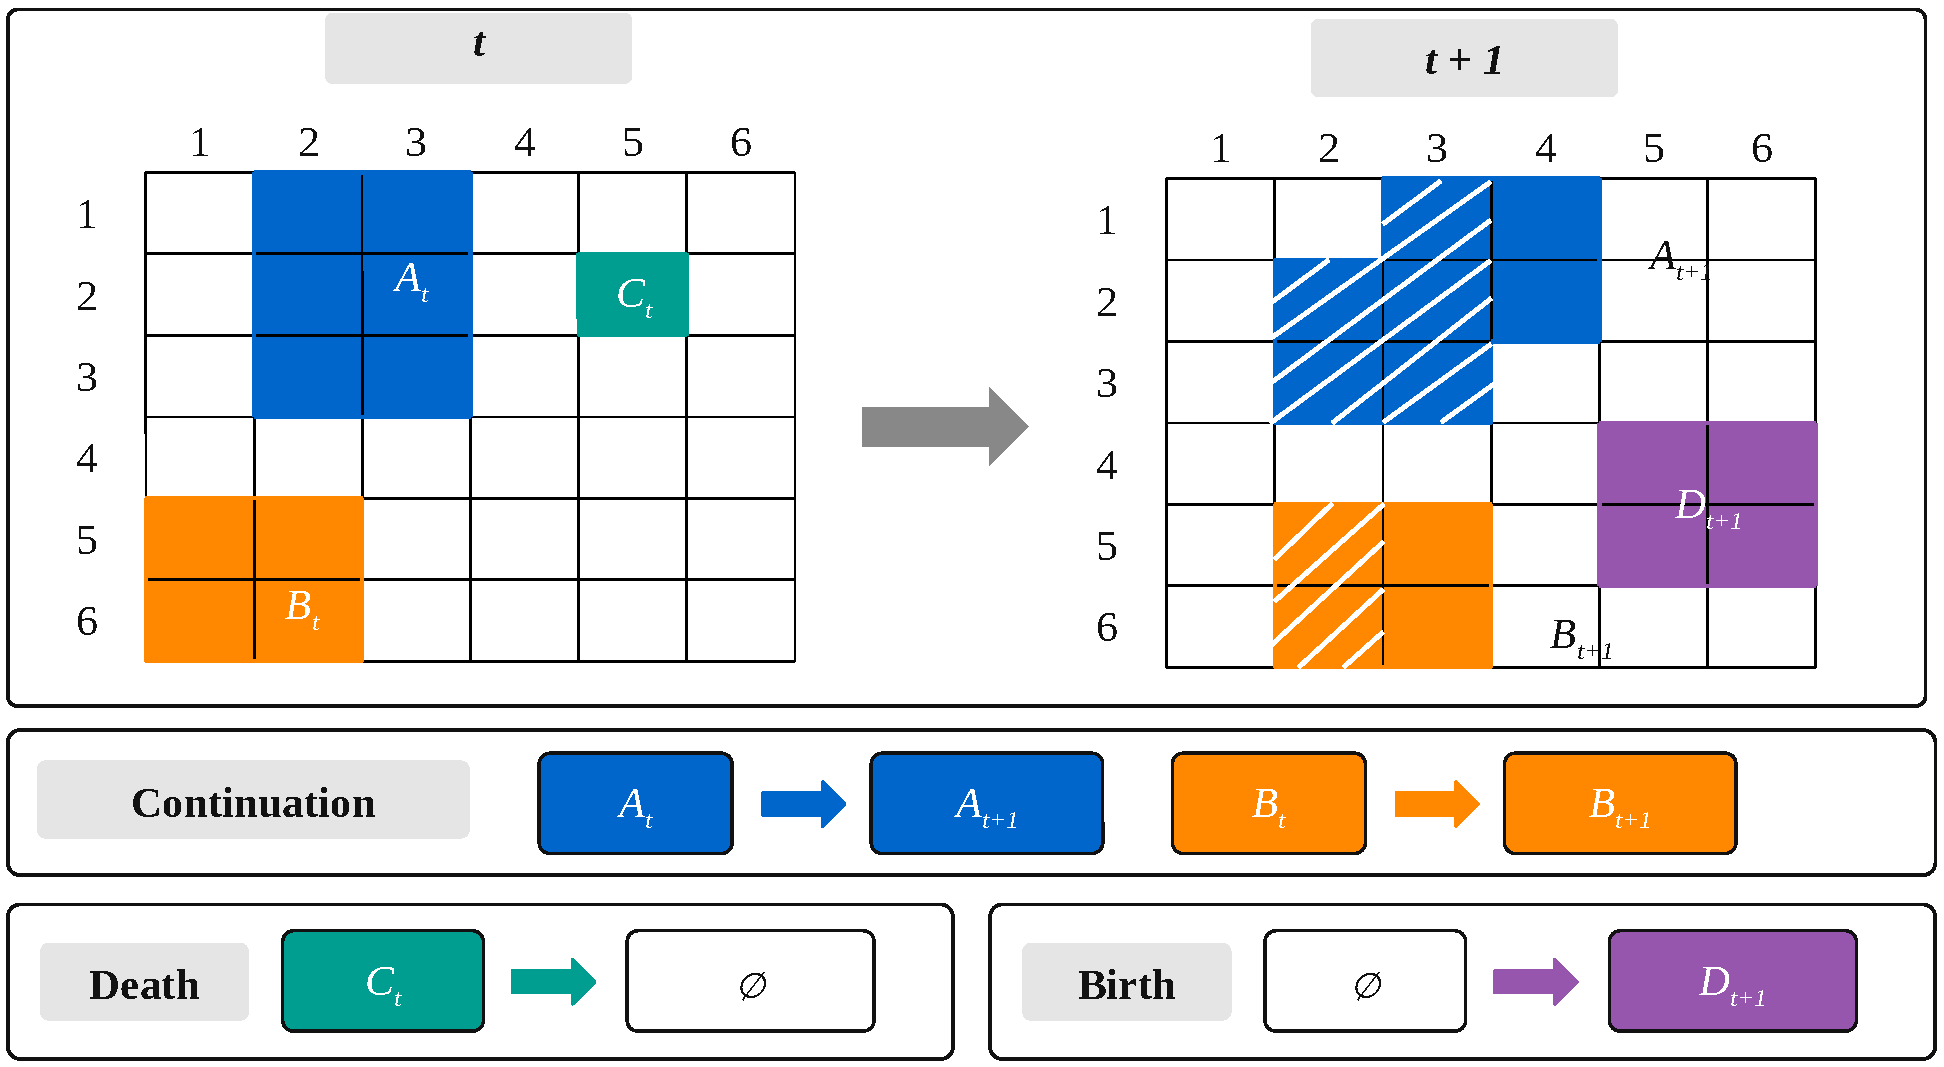
\includegraphics[width=\columnwidth]{figures/anchor_leaf_correspondence_v26.pdf}
\caption{Leaf correspondence across frames: leaf-arc supports are matched one to one by maximum overlap; matched leaves continue a track, unmatched ones start or end one.}
\label{fig:supp-correspondence}
\end{figure}
The paper describes the construction mathematically. The conventions below record how the implementation realizes it, including correspondence, reference estimation and the single-control interface.

\paragraph{Correspondence provenance and temporal confidence.}
The shared fixed-grid extractor in \texttt{experiments/era5.py} calls \texttt{match\_leaves\_by\_overlap} on consecutive augmented-tree frames. Supports contain the extremum and leaf-arc regular samples, excluding the parent critical sample. Stable \texttt{sample\_ids} identify common spatial samples; fixed-grid C-order indexing supplies them in this extractor. A Hungarian assignment maximizes total intersection count, and zero-overlap pairs are discarded. Matched leaves inherit Track IDs; unmatched current leaves receive new IDs. The first frame and declared temporal-window breaks start identities without a predecessor. Tied assignments have no additional physical tie-breaking criterion.

The shared 2D/3D extraction path and the native-volume paths must be distinguished. The latter accumulate intersections from original-voxel leaf-arc ownership arrays, exclude roots, and retain positive-overlap Hungarian pairs. They implement the same count-based assignment principle through different support representations, rather than all calling one matching function. The automatic-reference adapter accepts precomputed, row-aligned Track IDs and checks frame-wise uniqueness; it does not verify their upstream matching provenance. External inputs must therefore declare their support and correspondence conventions.

For a persistent ID present in consecutive frames, \texttt{motion\_pairs} supplies an extremum displacement to the single sequence-wide direction fit. Unmatched leaves and track interruptions supply no displacement for that step. Rapid motion, support changes or weak overlap may remove or alter correspondences and affect this fit. The implementation does not reconstruct physical split/merge events, branching lineages or links across missing frames.

For placement, the adapter and \texttt{solve\_unified\_sequence} align previous anchors and references by Track ID and pass a valid-match mask. They use unit temporal confidence. Shared preprocessing also records support IoU for diagnostics; the legacy ERA5 extremum-reference branch additionally passes it as \texttt{temporal\_confidence} to the low-level solver. That branch weights temporal residuals by IoU, but still maximizes intersection counts during matching. The current automatic-reference adapter does not enable this weighting; direction estimation also does not use IoU weights.

\paragraph{Automatic reference and implementation convention.}
The default preprocessing uses the leading eigenvector of the scatter of all matched extremum displacements, once over the full sequence in either 2D or 3D. It maximizes squared projected motion. The sign gives nonnegative total signed motion; when that sum is within $10^{-12}$ of zero, the largest-magnitude component is positive. If motion energy is at most $10^{-20}$, the longest domain axis is used, choosing the first on a tie. These are the existing \texttt{directional\_reference} conventions. A physical direction may be supplied. Repeated top eigenvalues need not select a unique direction; the relative eigengap is reported. This is standard spectral estimation, not joint optimization of direction and topology.

The projected bounding-box corners supply origin $o$ and span $L$. Code stores raw $p_i^t\cdot a$ on $[o,o+L]$; the paper uses $q_i^t=p_i^t\cdot a-o$ and translates anchors and centers by the same origin. Motion differences are invariant under this shift. The low-level \texttt{solve\_anchored\_sequence} adapter connects this preprocessing to the finite width-aware search and four-term capped QP. It returns continuous layouts; the public \texttt{anchor\_mtm} entry additionally invokes existing reconstruction and diagnostics, as specified below. Neither output is an unconditional raster certificate. Existing fixed-axis experimental drivers and stored evidence have not been rerun or relabelled as automatic-reference experiments.

\paragraph{Single-control configuration and execution.}
The public execution is \texttt{prepare\_fields} (or \texttt{prepare\_sequence}) followed by \texttt{anchor\_mtm(prepared, epsilon)}. Preprocessing and its fitted reference are reused for all budgets. The fixed numerical allowance is $\varepsilon_0=10^{-7}$; every order stage uses the same absolute $\eta=(\varepsilon_0+\varepsilon)\Delta_F$. Default $\varepsilon=0$ retains this allowance and is not strict Exact Mode. Zero labelled error is the mathematical case $\eta=0$, obtained with both allowances zero. Neither 20\% nor 100\% limits the interface.

The default configuration uses the existing scale rules: width scale $s=0.5L/\operatorname{measure}(D)$, gap $g=L/240$, position slack $\beta_0=L/120$, $\rho=0.5$, and weights $(\lambda_R,\lambda_M,\lambda_G,\lambda_C)=(4,0.5,1,0.1)$. All are fixed for a prepared sequence. Output resolution defaults to 2048 samples; insufficient raster capacity is a reported failure. Advanced fixed configurations retain these quantities rather than deleting constraints. Reference-aligned motion and term means are the default. An independently supplied reference cap or conflicting motion control is rejected by the new placement interface.

The canonical ordering implementation retains the existing threshold/selective flattening, midpoint and block-insertion strategies (four initial refinement seeds plus the exact tree, at most eight refinement passes). A collector records generated initial and trial permutations, retaining strict-tree orders and the point candidate. The deduplicated finite pool is evaluated for $\delta^*$, $\tau$ and NROE, filtered by $\eta$, then selected lexicographically by $(\tau,\mathrm{NROE})$; an exact tie uses the permutation lexicographically for reproducibility. The QP receives a singleton order and the explicit cap $\tau+\beta_0$. The older general-purpose \texttt{Controls} interface can use an absolute position cap and compare multiple orders by QP objective; it is not the default AnchorMTM entry. Historical experiment drivers and their outputs are unchanged.

Reconstruction calls the existing leaf/LCA filling and optimal-barrier correction. Records include candidate totals and admitted counts, selected order, $\tau$, $\delta^*$, anchors, reference displacement, NROE, continuous motion residual, and separately rendered errors and failures. NMLEmean and NMLEmax use absolute error over the full fixed-label merge matrix (including the diagonal), divided by $\Delta_F$; ME is the RMS reference-motion residual divided by $L$. Rendered motion is also measured at rounded anchors. A successful computation may record a rendered budget violation; it does not certify full-tree label coverage or repair the output. The renderer's strict-extremum clearance remains separate from the continuous optimum.

\FloatBarrier
\section{Compared Methods, Data and Settings}\label{sec:protocol}
\subsection{Methods as Instances of One Layout Problem}\label{sec:family}
\begin{figure*}[t]
\centering
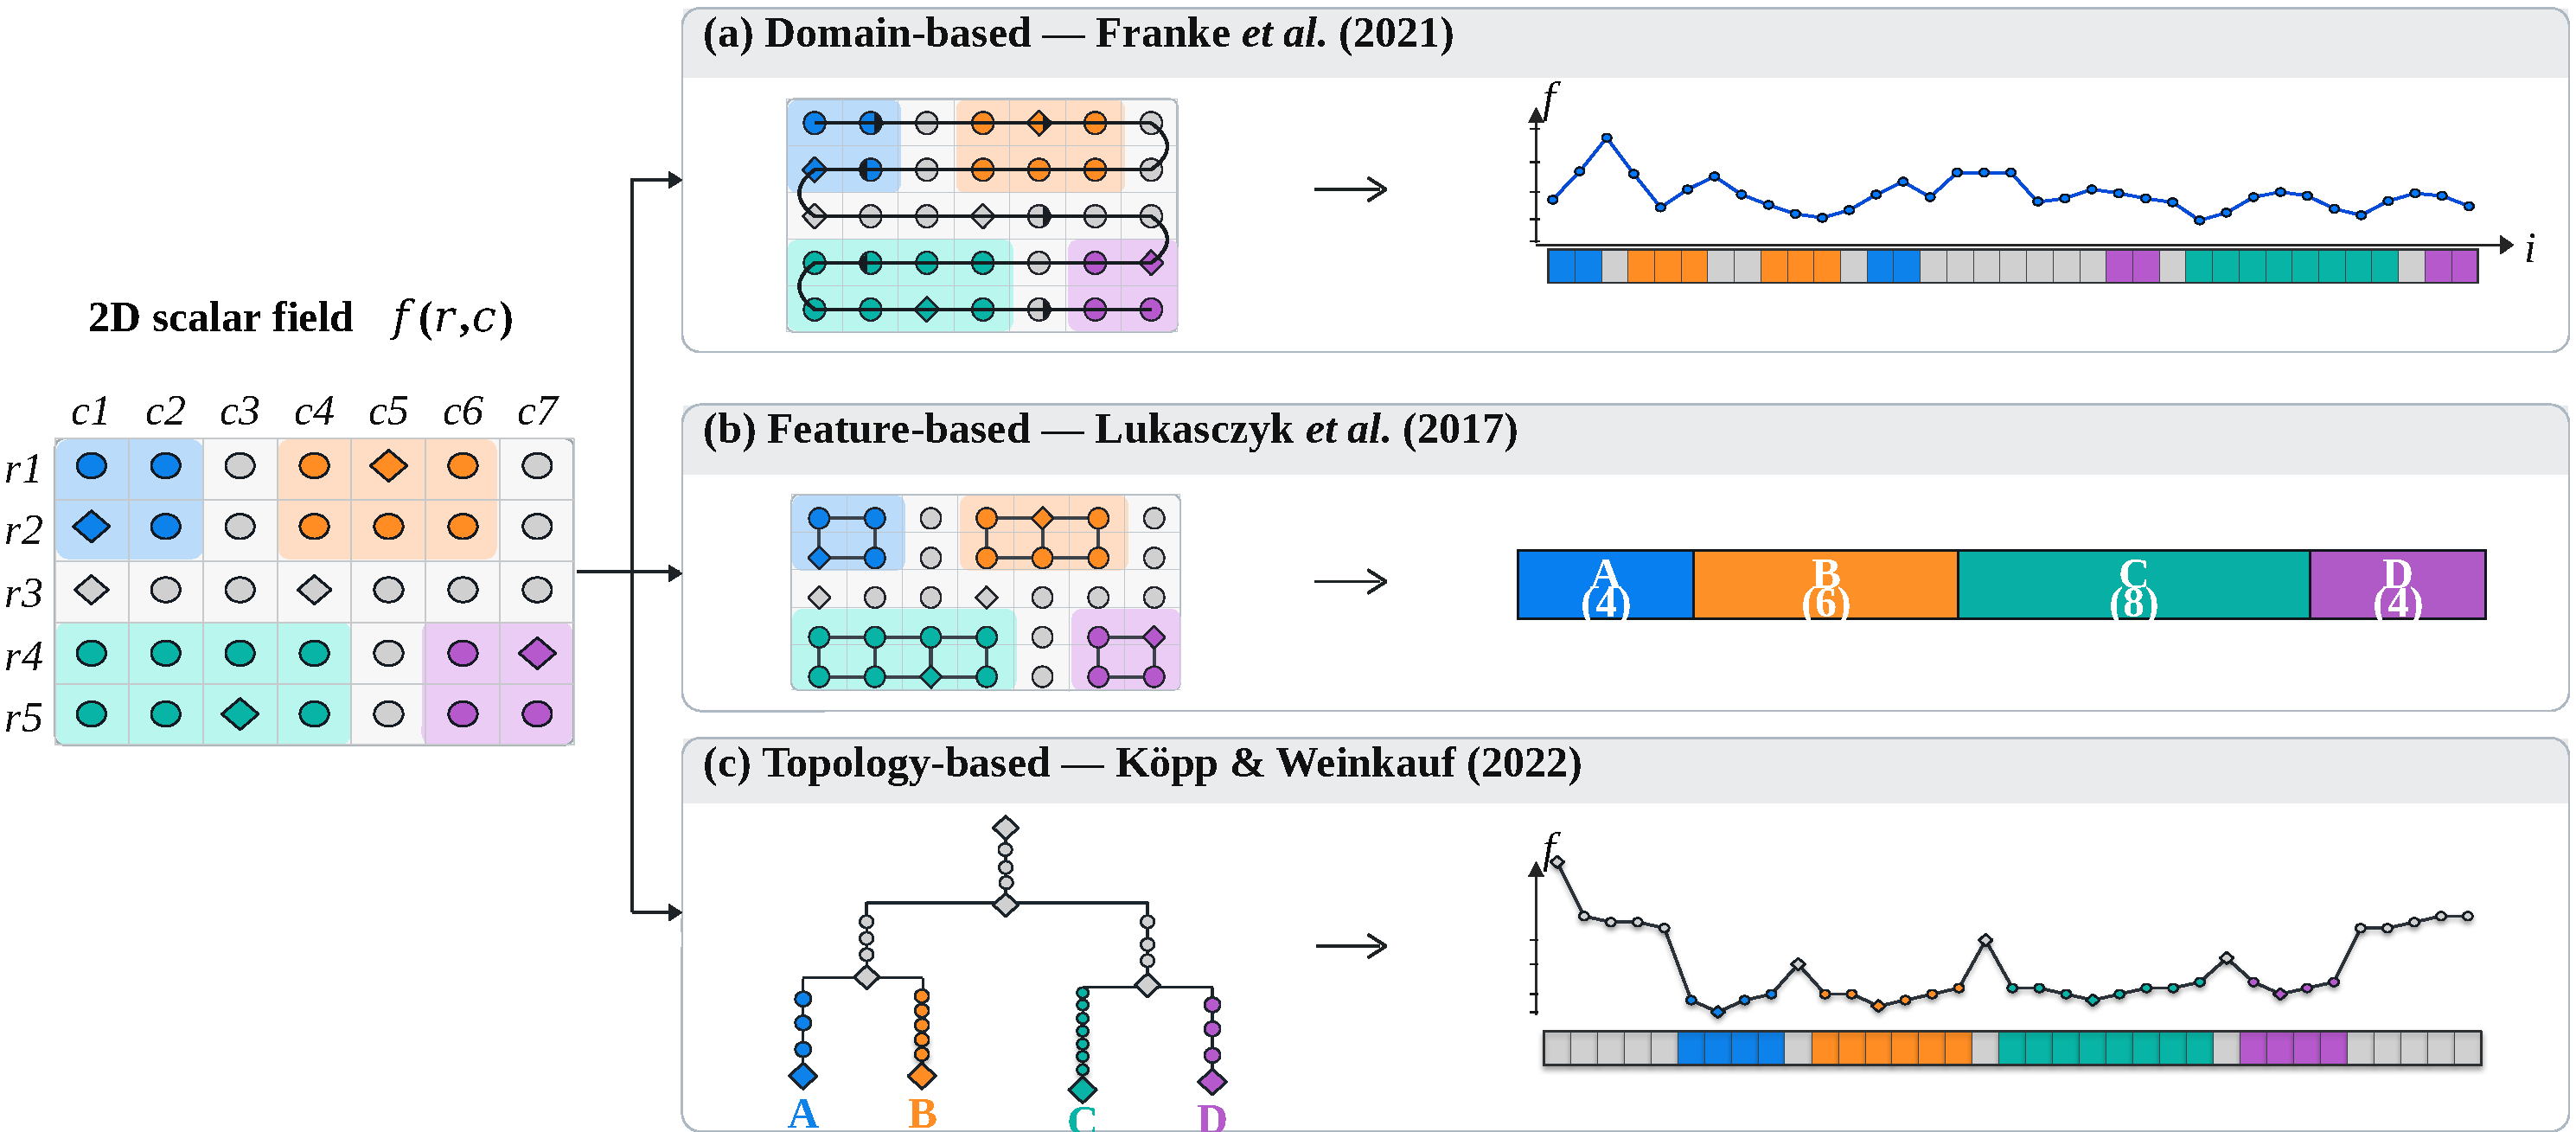
\includegraphics[width=.92\textwidth]{figures/anchor_related_work_mapping_v26.pdf}
\caption{Three ways to draw a scalar field along one axis, on a common 35-sample field. (a) Domain-based traversals keep sample adjacency along a curve; (b) feature-based summaries keep feature sizes; (c) topology-based profiles keep the merge tree. AnchorMTM belongs to (c) and adds a fixed spatial direction to it.}
\label{fig:supp-mapping-strategies}
\end{figure*}
\begin{table}[t]
\centering
\caption{Maps of time-varying scalar fields as instances of the layout problem (Eq.~3 of the paper). Order rule: how leaves are ordered; placement: nonzero terms and temporal target; $\eta$: allowed merge error relative to the scalar range (tolerance $\varepsilon_0$ omitted); axis: what a position encodes.}
\label{tab:family}
\footnotesize
\setlength{\tabcolsep}{2pt}
\renewcommand{\arraystretch}{1.05}
\begin{tabular*}{\columnwidth}{@{\extracolsep{\fill}}>{\raggedright\arraybackslash}p{0.19\columnwidth}>{\raggedright\arraybackslash}p{0.25\columnwidth}>{\raggedright\arraybackslash}p{0.25\columnwidth}c>{\raggedright\arraybackslash}p{0.13\columnwidth}@{}}
\toprule
Method & Order rule & Placement & $\eta$ & Axis \\
\midrule
TMTM~\cite{Koepp:2023:TMTM} & greedy child order by subtree overlap between frames & packed by sample count; no anchor optimization & 0 & tree traversal \\
ST-MTM~\cite{STMTM:2026} & concordant order unless OLO is cheaper by a ratio & $\lambda_G$ (stress), $\lambda_M$ on matched anchors, then intervals & 0 & relative distance \\
OLO~\cite{BarJoseph:2001:OLO} & tree-constrained OLO & ranks only & 0 & order \\
Projection, Hilbert, Morton~\cite{Franke:2021:1DP} & by reference or curve & at reference or curve rank & none & location or curve rank \\
\midrule
AnchorMTM & least $\tau$ within the budget & $\lambda_R$ dominant, $\hat x$ follows projected motion & $\varepsilon$ & location \\
\bottomrule
\end{tabular*}
\end{table}

The layout problem of the paper (Eq.~3) chooses a leaf order and a placement under a merge-error limit $\eta$. Table~\ref{tab:family} places every compared method in this problem. TMTM and ST-MTM keep the tree ($\eta=0$) and have no reference term, so their axes encode a tree traversal or relative distances. OLO keeps the tree and only orders leaves, so it is measured by order error alone. The projection and the space-filling curves follow space and ignore the tree. AnchorMTM adds the reference term and the declared allowance. The correspondence concerns the problem each method solves; solvers differ in scaling and other details, and the evaluation uses implementations of the published methods, not our solver with their weights.

\subsection{Baseline Implementations and Orientation}\label{sec:baselines}
TMTM is a port of its official implementation and matches its core in all 3127 arc intervals and anchors of the planar bound sequences. ST-MTM has no public code; our implementation follows its published description with temporal reordering threshold $0.95$ and meets the optimality conditions of its quadratic programs (relative KKT residuals below $10^{-6}$). On the hourly Storms archive of the paper's Fig.~1, genuine multiway saddles are handled by equal-level separators in TMTM and by an equal-level binary refinement in ST-MTM whose leaf merge matrices are checked. On PM$_{2.5}$, ST-MTM uses the published Storms parameters. Hilbert and Morton curves keep a fixed grid orientation in the layout-suite table.

A merge tree map without a reference has no preferred direction: its mirror image is an equally optimal output of the same method. Each baseline in the layout-suite table is therefore reflected once for the whole sequence if its anchors and references correlate negatively on the first frame where both vary; on PM$_{2.5}$ this reflects TMTM but not ST-MTM. The bound-suite results and the volume figure use the global mirror that agrees better with the reference over the whole sequence. Over all temporal reordering thresholds from 0 to 1, each in its favourable mirror, the share of ST-MTM's order error not forced by the tree stays within 53--95\% on the real planar bound sequences and within 37--61\% on Ring.

On the four benchmark inputs, the SNS and TW of TMTM and ST-MTM are quoted from the ST-MTM paper (Temporal mode, authors' inputs) and are not ranked against local values. Local TW uses $k=(1,3,5,3)$ on Gaussian, Ring, Wildfires and Storms, counting only frames with $0<k<n_t/2$ (64/64, 1/40, 4/32 and 11/744), and $k=1$ on all 744 PM$_{2.5}$ frames.

\subsection{Data Preparation}\label{sec:dataprep}
The \emph{bound suite} reuses the saved trees, matches and references of an earlier benchmark, prepared with one extractor, one matching rule and one reference estimator, and laid out with one default configuration $\Theta_0$ on every sequence. Its 12-hourly Storms and 30-frame Wildfires sequences are prepared differently from the hourly Storms and 32-frame Wildfires inputs of the layout suite, and Ring follows the TMTM generator.

The \emph{layout suite} reconstructs the four planar inputs of the ST-MTM benchmark. Author-processed arrays are unavailable, so the persistence values of ST-MTM are read as per-frame range fractions (0.1, 0.1, 15 and 10.5\% for Gaussian, Ring, Wildfires and Storms); the result is a disclosed reconstruction, not an identical-input reproduction. The hourly PM$_{2.5}$ sequence covers January 2017 over northern China (110--120$^\circ$E, 32--41$^\circ$N) with 744 reanalysis fields interpolated to $160\times144$. Its maxima are extracted as join trees of the negated field with a persistence of 5\% of each frame's range, a threshold independent of the 5\% layout budget. The volumetric inputs are listed in Table~\ref{tab:volume-parameters}.

\subsection{Settings, Budget Selection and Runtime}\label{sec:settings}
\begin{table}[!ht]
\centering
\caption{Planar parameter settings and runtime (seconds): Balanced on the benchmark inputs, a fixed 5\% budget on PM$_{2.5}$.}
\label{tab:anchor-parameters-final}
\footnotesize
\setlength{\tabcolsep}{2pt}
\renewcommand{\arraystretch}{0.95}
\begin{tabular}{@{}lccccc@{}}
\toprule
Parameter & Gaussian & Ring & Wildfires & Storms & PM$_{2.5}$ \\
\midrule
$\varepsilon$ & 1\% & 1\% & 5\% & 10\% & 5\% \\
$N_r$ & 4096 & 196 & 4096 & 4096 & 4096 \\
$s_w$ & 0.00581 & 0.00328 & 0.00053 & 0.01170 & 0.00073 \\
$t_{opt}$ & 0.156 & 0.150 & 3.324 & 2.600 & 199.975 \\
$t_{total}$ & 1.340 & 0.486 & 4.424 & 63.447 & 231.177 \\
\bottomrule
\end{tabular}
\vspace{2pt}
\begin{minipage}{0.94\columnwidth}\footnotesize Weights $(4,1,0.5,0.1)$ and $\rho=0.5$ are fixed. $s_w$ is width per support measure; $N_r$ is raster length. Times are one uncached run on Apple M4: optimization and full pipeline, respectively.\end{minipage}
\end{table}

\begin{table}[t]
\centering
\caption{Volumetric datasets and Balanced-mode parameter settings.}
\label{tab:volume-parameters}
\footnotesize
\setlength{\tabcolsep}{2pt}
\renewcommand{\arraystretch}{0.95}
\begin{tabular}{@{}lcc@{}}
\toprule
Parameter & Cylinder & Tangaroa \\
\midrule
Frames & 102 & 201 \\
Grid & $135\times64\times48$ & $300\times180\times120$ \\
Scalar & $Q$-criterion & Speed $\|\mathbf{v}\|$ \\
Persistence & 2\% per-frame range & 0.2 absolute \\
Reference & $+x$ & $+x$ \\
$\varepsilon$ & 1\% & 33.33\% \\
$L$ & 32768 & 131072 \\
$s_w$ & $2.70668\times10^{-5}$ & 0.40953 \\
Weights & $(0.1,16,0,0.1)$ & $(0,64,0,0)$ \\
$\rho$ & 1 & 1 \\
Gap$/L_{world}$ & $1/300$ & $1/960$ \\
Extra$/L_{world}$ & 0.1 & 0.1 \\
\bottomrule
\end{tabular}
\vspace{2pt}
\begin{minipage}{0.94\columnwidth}\footnotesize Weights are reference, geometry, temporal and eccentricity. $s_w$ is width per support measure (Cylinder voxel counts; Tangaroa physical volume); $L$ is raster length, distinct from the physical canvas extent $L_{world}$. Exact uses zero allowance with the same other parameters as its Balanced counterpart.\end{minipage}
\end{table}

Table~\ref{tab:anchor-parameters-final} lists the four planar Balanced budgets (1, 1, 5 and 10\%), the fixed 5\% budget of the hourly PM$_{2.5}$ sequence and the layout parameters; Table~\ref{tab:volume-parameters} separately lists the volumetric datasets and settings. The planar table reports one uncached run per sequence on Apple M4, with one BLAS/TTK thread, sequential extraction and the default HiGHS scheduler. Optimization includes ordering and placement; total time additionally includes preprocessing, trees, matching/reference estimation, rasterization, I/O and checks. Imports, reporting and metric export are excluded; OS caches may be warm. Timings do not establish speedup significance. Baseline NPE uses the disclosed CompactTMTM and ST-MTM solver adaptations, not author binaries.

The Balanced budget of each planar input was chosen once from 1--10\% on the first chronological quarter of the sequence by $J=0.5\,\mathrm{NPE}_{norm}+0.5\,\mathrm{SNS}_{norm}$ over candidates within their budget, preferring smaller budgets within 0.01 of the minimum, and frozen before the full runs. Earlier outputs had been observed, so this is not a blind test. PM$_{2.5}$ was added later with a fixed budget of 5\% that this rule did not select, and it is reported under its budget. The volumetric table of the paper uses the stored configurations of Table~\ref{tab:volume-parameters} with the $+x$ reference chosen by an offline displacement rule; the volume figure and the per-frame distributions use the default configuration of the bound suite.

\begin{figure*}[t]
\centering
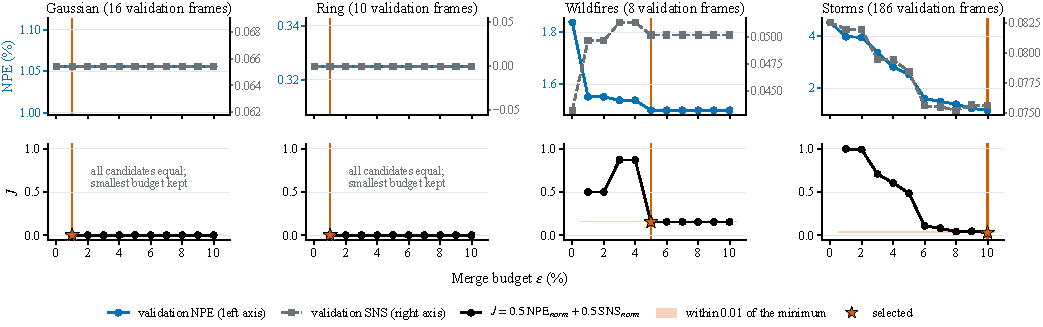
\includegraphics[width=\textwidth]{figures/budget_supp_selection.pdf}
\caption{Selection of the Balanced budget on the first chronological quarter of each sequence (validation frames). Top: validation NPE (left axis) and SNS (right axis) for $\varepsilon=0$--10\%. Bottom: the score $J$ of the paper over the eligible positive budgets, the band within 0.01 of its minimum, and the selected budget (star), frozen before the full runs. On the Gaussian and Ring validation frames every candidate gives the same map, so the smallest budget is kept.}
\label{fig:supp_budget_selection}
\end{figure*}

Figure~\ref{fig:supp_budget_selection} shows this selection rule. On Wildfires 5\% gives the smallest validation NPE at a small SNS cost and is the smallest budget within the tolerance; on Storms validation NPE falls at every step up to 10\%, SNS changes little beyond 6\%, and $J$ is smallest at 10\%. The first quarter of Ring contains no conflict that a budget releases (Fig.~\ref{fig:supp_budget_matrix}), so its selection keeps 1\%, while later frames change at larger budgets.

\FloatBarrier
\section{Additional Results}\label{sec:results}
The results below follow the evaluation of the paper: tightness and forced error (S5.1), maps and positions on every sequence (S5.2), the per-frame effect of the budget (S5.3), and three qualitative cases (S5.4--S5.6).

\subsection{Tightness of the Bounds and Forced Error}\label{sec:supp_bounds}
The paper evaluates the bounds on the bound suite (Section~\ref{sec:dataprep}). Table~\ref{tab:supp_bounds} lists the sequences and, for four budgets, the frames on which the interval cost $\tau$ of the selected order equals the lower bound; for $\varepsilon>0$ the bound is the larger of the bounded-topology certificate and the flattening certificate (Section~\ref{sec:chain}).

\begin{table*}[t]
\centering\small
\caption{Earlier benchmark and bound attainment: frames on which $\tau$ of the selected order equals the lower bound. Leaves: retained extrema per frame.}\label{tab:supp_bounds}
\begin{tabular}{llrrlrrrr}\toprule
Sequence & Scalar field & Frames & Leaves & Tree & $\varepsilon=0$ & 2\% & 5\% & 10\%\\\midrule
Storms & ERA5 sea-level pressure, 2D & 118 & 1--8 & join & 116 & 116 & 110 & 110\\
Wildfires & $\log(1+\mathrm{FRP})$, 2D & 30 & 6--11 & split & 25 & 27 & 24 & 24\\
OLR & outgoing longwave radiation, 2D & 60 & 2--8 & join & 60 & 60 & 60 & 59\\
PM$_{2.5}$ & PM$_{2.5}$ concentration, 2D & 366 & 1--7 & split & 365 & 361 & 363 & 363\\
Ring & synthetic ring intensity, 2D & 40 & 1--7 & split & 40 & 40 & 40 & 40\\\midrule
\multicolumn{2}{l}{Planar total} & 614 & & & 606 & 604 & 597 & 596\\\midrule
Tangaroa & velocity magnitude, 3D & 201 & 18--93 & join & 27 & 24 & 30 & 24\\
Cylinder & $Q$ criterion, 3D & 102 & 4--75 & split & 81 & 77 & 76 & 74\\\bottomrule
\end{tabular}
\end{table*}

Table~\ref{tab:supp_forced} splits the order error of the three tree-keeping maps on the same frames. All three keep the merge tree exactly, so Theorem~1 of the paper applies: midpoint ordering of the same tree attains $\nu^*$, and the share of the mean NROE above the mean $\nu^*$ is chosen by the order rule rather than forced by the hierarchy. Shares are computed from unrounded means, each map in the mirror that agrees better with the reference.

\begin{table}[h]
\centering\small
\caption{Order error of the tree-keeping maps on the bound suite (percent of the canvas, means over frames) and the share above the strict bound $\nu^*$.}\label{tab:supp_forced}
\setlength{\tabcolsep}{3pt}
\begin{tabular}{lrrrrrrr}\toprule
 & & \multicolumn{2}{c}{OLO} & \multicolumn{2}{c}{TMTM} & \multicolumn{2}{c}{ST-MTM}\\\cmidrule(lr){3-4}\cmidrule(lr){5-6}\cmidrule(lr){7-8}
Sequence & $\nu^*$ & NROE & share & NROE & share & NROE & share\\\midrule
Storms & 3.77 & 15.60 & 76 & 18.31 & 79 & 16.28 & 77\\
Wildfires & 5.80 & 19.06 & 70 & 19.65 & 70 & 18.72 & 69\\
OLR & 0.89 & 16.27 & 95 & 19.31 & 95 & 16.59 & 95\\
PM$_{2.5}$ & 0.97 & 5.17 & 81 & 4.44 & 78 & 5.21 & 81\\
Ring & 2.66 & 4.23 & 37 & 7.18 & 63 & 4.47 & 41\\
Tangaroa & 9.24 & 15.44 & 40 & 19.50 & 53 & 15.80 & 41\\
Cylinder & 12.24 & 18.03 & 32 & 26.62 & 54 & 17.77 & 31\\\bottomrule
\end{tabular}
\end{table}

The position--topology plane of the paper (Fig.~5) evaluates the bound on 126 allowances and the AnchorMTM order on 43, both without numerical allowance, so at $\varepsilon=0$ the bound is the strict $\nu^*$; at the nine allowances of Table~\ref{tab:supp_bounds} the computation reproduces the saved results exactly. At $\varepsilon=0$ the AnchorMTM order attains $\nu^*$ on all 917 frames. The shape of the edge follows Theorem~3 of the paper: where conflicting subtrees merge just below their parent, a small allowance releases them (Wildfires: 5.80\% to 2.77\% at 1\%; Cylinder: 12.24\% to 0.23\% at 1\%, and to 6.15\% already below $10^{-6}$ of the scalar range, the precision of the stored data), while deep conflicts stay expensive (Tangaroa above 7\% up to 5\%; Storms 1.43\% at 10\%). On Storms, OLR, daily PM$_{2.5}$ and Ring every frame has at most eight leaves; enumerating all leaf orders shows that the AnchorMTM order is the exact optimum at every tested allowance, except one Storms frame at $\varepsilon=31.6\%$ (1.9 percentage points).

Because the bounds need no layout, they can also compare reference directions before any map is drawn (Fig.~\ref{fig:supp_direction}).
\begin{figure}[t]
\centering
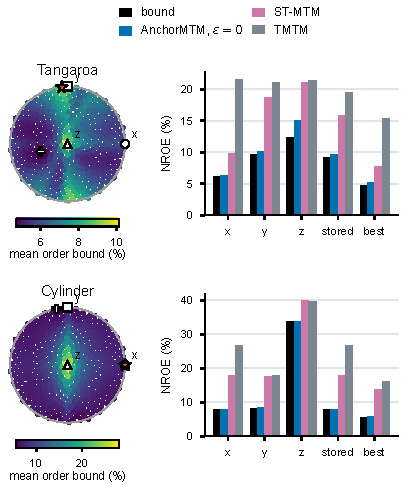
\includegraphics[width=\columnwidth]{figures/supp_direction.pdf}
\caption{The forced cost depends on the reference direction and can be computed before a map is drawn. Left: mean order bound at the numerical allowance $\varepsilon_0$ over 400 directions of the hemisphere (equal-area projection; centre $z$, rim the $xy$ plane); markers: coordinate axes, the stored direction (star) and the smallest bound (cross). Right: the bound and the mean order error of AnchorMTM at $\varepsilon=0$, ST-MTM and TMTM in these directions. The bound spans 4.70--10.14\% on Tangaroa and 5.49--28.15\% on Cylinder.}
\label{fig:supp_direction}
\end{figure}

\FloatBarrier
\subsection{Maps and Positions on Every Sequence}\label{sec:supp_positions}
\begin{figure*}[t]
\centering
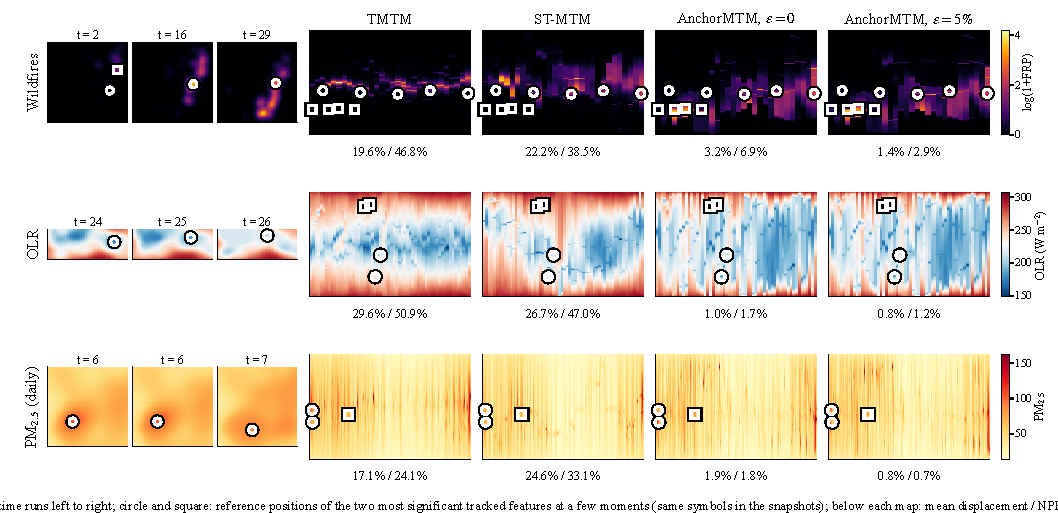
\includegraphics[width=\textwidth]{figures/map_gallery_supp.pdf}
\caption{Rendered maps of OLR and daily PM$_{2.5}$, encoded as the map figure of the paper: three tracked extrema per sequence (circles in the snapshots, dashed reference trajectories on the maps). On PM$_{2.5}$ the tracked maxima move little and the matched identities change often, so its maps look alike; the positional difference shows in the numbers below each map.}
\label{fig:supp-map-gallery}
\end{figure*}
\begin{figure*}[t]
\centering
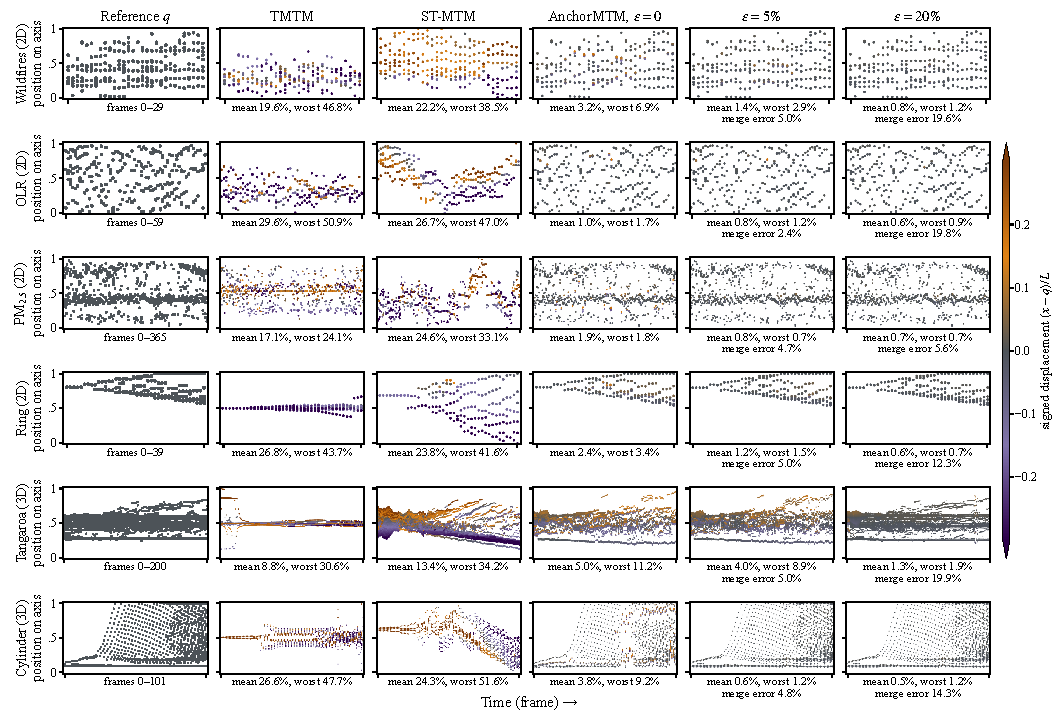
\includegraphics[width=\textwidth]{figures/volume_gallery.pdf}
\caption{Every extremum against its reference, on four planar and two volumetric sequences. Each dot is one extremum in one frame at its position on the axis (fraction of the canvas), coloured by its signed displacement $(x-q)/L$; grey dots lie on their references. The first column shows the references themselves. Native maps are rescaled to the canvas, in the mirror that agrees better with the reference; AnchorMTM uses the default configuration. Below each panel: mean displacement, mean worst displacement per frame and, for a positive budget, the attained merge error.}
\label{fig:supp-positions}
\end{figure*}
The map figure of the paper follows a few tracked features; Figs.~\ref{fig:supp-map-gallery} and~\ref{fig:supp-positions} show the rest. Figure~\ref{fig:supp-positions} plots every extremum of every frame, so it shows the whole distribution of displacements rather than selected features. On the four planar sequences, TMTM and ST-MTM draw extrema 17--30\% of the axis from their references on average, AnchorMTM with the exact tree 1.0--3.2\%. On Cylinder, TMTM and ST-MTM gather the vortices near the middle of the axis, whereas AnchorMTM already reproduces the shedding pattern of the references with the exact tree; on Tangaroa, whose conflicts lie deep in the tree, the pattern appears only near $\varepsilon=20\%$. Table~\ref{tab:full-planar-positions} and Table~\ref{tab:full-volume} list the numbers.

\FloatBarrier
\subsection{Where a Budget Acts}\label{sec:supp_budget}
The tables of the paper report means over frames; the figures of this subsection show the frames behind them. The planar runs cover the complete sequences with the references, widths, gaps, weights and raster lengths of the paper's four-dataset comparison table, and only $\varepsilon$ changes. The run at $\varepsilon=0$ is Exact Mode and the run at the selected budget (Ring 1\%, Wildfires 5\%, Storms 10\%) is Balanced Mode; both coincide value by value with the table runs. For frame $t$, the worst displacement is $\max_i|x_i^t-q_i^t|/L_{world}$ on rendered anchors, and its mean over frames is the table's NPE; the merge error is the attained fixed-leaf merge error, including diagonal extrema, divided by the scalar range; SNS is the frame's scale-normalized stress. Every run passes its continuous and rendered budget checks. Gaussian gives the same map at every budget and is omitted.

\begin{figure*}[t]
\centering
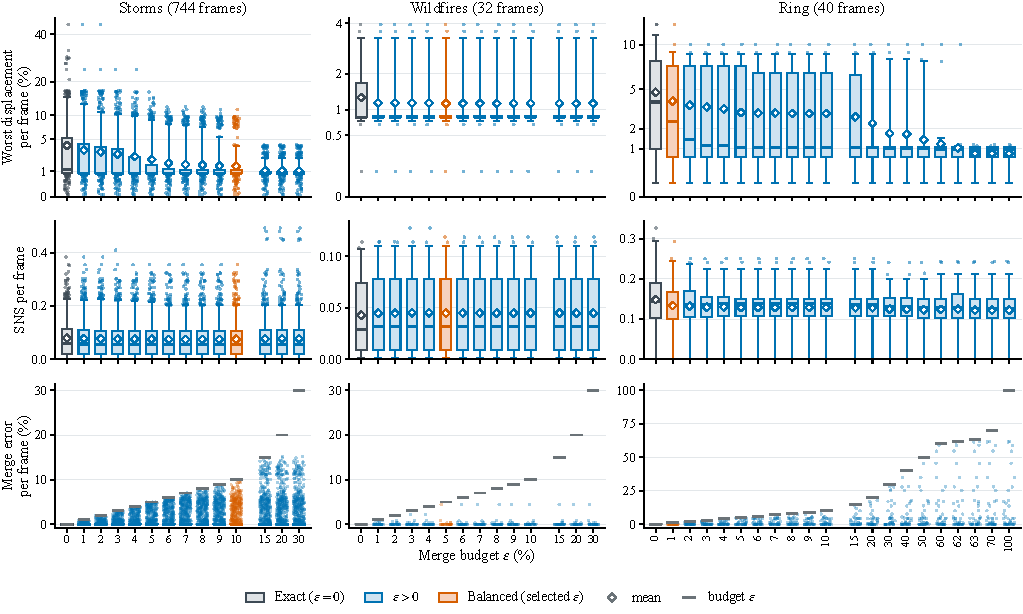
\includegraphics[width=\textwidth]{figures/budget_supp_extended.pdf}
\caption{Per-frame distributions over the complete budget sweep. Rows: worst displacement per frame (square-root scale), SNS per frame (frames with too few features omitted), and attained merge error per frame with its budget (grey dash). Budgets above 10\% use larger steps (gap in the axis); Ring is swept to 100\% to locate its last release. Boxes: quartiles; whiskers: 5th--95th percentiles; dots: other frames; diamonds: means.}
\label{fig:supp_budget_extended}
\end{figure*}

Figure~\ref{fig:supp_budget_extended} extends the sweep of the paper to 30\% (Ring 100\%) and adds SNS. On Storms the upper tail keeps shrinking up to 15\%, where the worst frame reaches 4.08\%, and nothing changes beyond; 294 of 744 frames then use the allowance. SNS is a by-product rather than a target of the budget: it falls on Ring (0.149 at $\varepsilon=0$, 0.129 at 10\%) and slightly on Storms (0.079 to 0.074 at 10\%, 0.076 from 15\%), but rises on Wildfires (0.043 to 0.045). On Ring the last frame keeps a displacement of 10.02\% until $\varepsilon=63\%$; enumerating all 120 orders of that five-leaf frame places its continuous release threshold at 62.0014\%.

\begin{figure*}[t]
\centering
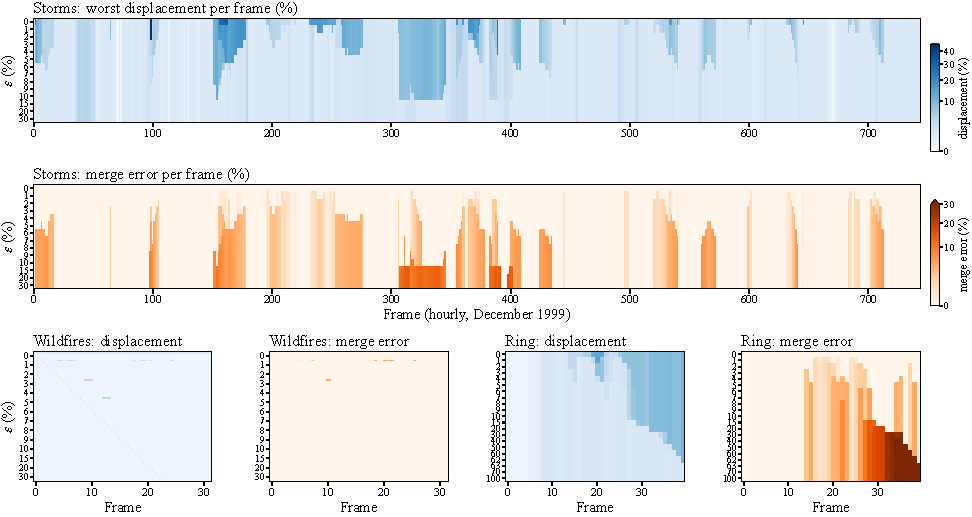
\includegraphics[width=\textwidth]{figures/budget_supp_matrix.pdf}
\caption{Which frames change. Each row is one budget and each column one frame; colour gives the worst displacement (blue) or the attained merge error (orange) of that frame. Square-root colour scales are shared by all panels; merge errors above 30\% (Ring only) saturate. Storms frames are hourly from 1 to 31 December 1999.}
\label{fig:supp_budget_matrix}
\end{figure*}

Figure~\ref{fig:supp_budget_matrix} shows which frames change. The 294 Storms frames that use the allowance at some budget form 24 runs of consecutive hours, and the budget at which a frame first changes differs within a run. The two runs whose worst displacement still exceeds 9\% at $\varepsilon=10\%$, frames 151--177 and 305--345, are released at 15\%. All other frames keep the Exact layout at every budget.

\begin{figure}[t]
\centering
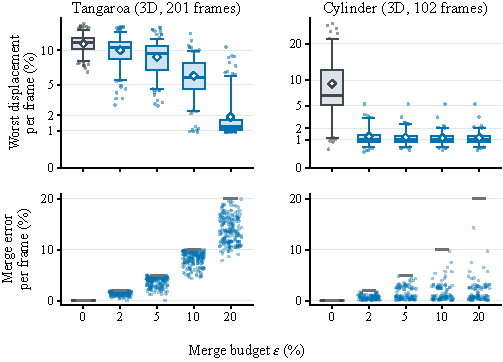
\includegraphics[width=\columnwidth]{figures/budget_supp_volume.pdf}
\caption{Volumetric budget sweeps with one default configuration: weights $(4,1,0.5,0.1)$, $\rho=0.5$, 8192-position rasters, and references from matched-extremum motion (Tangaroa) or the streamwise $x$ axis (Cylinder). These settings differ from the tuned configurations of the paper's volumetric table. All 1,515 rendered frames were rechecked against the fixed-leaf merge matrices; none exceeds its budget. Encodings as in Fig.~\ref{fig:supp_budget_extended}.}
\label{fig:supp_budget_volume}
\end{figure}

In the volumes almost every frame contains a conflict that a budget can release (Fig.~\ref{fig:supp_budget_volume}): 200 of 201 Tangaroa frames at 2\% and 5\% and all of them from 10\%, and 98 of 102 Cylinder frames at every positive budget. The whole distribution therefore moves. The Cylinder median falls from 6.76\% to 1.04\% already at 2\%, while the Tangaroa median falls gradually from 11.32\% to 1.20\% at 20\%, in line with its deep conflicts (Section~\ref{sec:supp_bounds}).



\FloatBarrier
\subsection{Reading an Air-Pollution Episode}\label{sec:supp_pm25}
\begin{figure}[t]
\centering
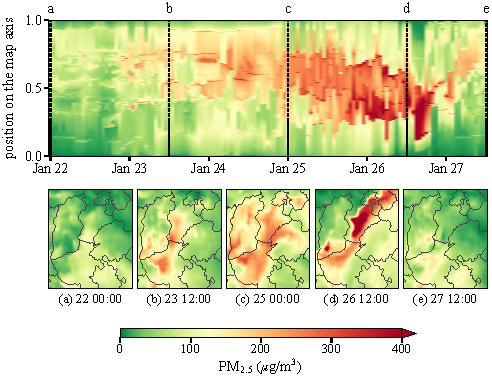
\includegraphics[width=\columnwidth]{figures/pm25_hourly.pdf}
\caption{An air-pollution episode in the hourly PM$_{2.5}$ sequence, 22--27 January 2017 (Beijing time), drawn by AnchorMTM with $\varepsilon=5\%$. Top: 133 hourly columns; dashed lines a--e mark the times of the snapshots below. Bottom: source fields over northern China. Concentrations above 400\,$\mu$g/m$^3$ saturate.}
\label{fig:pm25-hourly}
\end{figure}
Figure~\ref{fig:pm25-hourly} shows how a spatially anchored map reads an episode that the source fields confirm. On 22 January the air is clean (a). On 23 January, orange bands appear in the upper half of the map, and the source field shows separate pollution maxima (b). By 25 January the polluted area covers much of the region, and the bands widen (c). The episode peaks on 26 January: the highest concentrations lie in a narrow belt (d), and the darkest bands descend on the map, that is, the strongest maxima move toward lower reference positions. By 27 January the air has largely cleared (e). Because the axis is anchored, a band that keeps its height is a maximum that stays at the same position along the reference direction while its concentration changes, and a band that drifts is a maximum that moves along this direction. The merge error stays within the budget in all 744 frames (at most 4.998\%). The run stores no reference direction, so the snapshots carry no direction arrow, and no baseline layout of this sequence is available for a side-by-side view.


\subsection{Ring: Guidance and Budget Together}\label{sec:supp_ring_params}
\begin{figure}[!t]
\centering
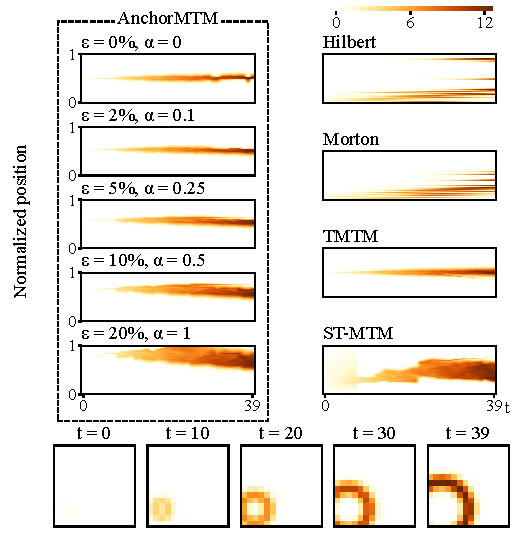
\includegraphics[width=\columnwidth]{figures/anchor_ring_result.pdf}
\caption{Ring comparison. Left: AnchorMTM with topology allowance $\varepsilon$ and guidance strength $\alpha=\varepsilon/20\%$ raised together, from neutral central targets ($\alpha=0$) to full spatial guidance ($\alpha=1$); the upward shift reflects guidance, not the allowance alone. Right: supplied Hilbert/Morton reference panels and same-input local TMTM/ST-MTM results. Below: source snapshots at frames 0, 10, 20, 30 and 39. All computed maps use 40 frames and 196 positions; the scalar key applies to computed maps and snapshots. Vertical coordinates denote normalized layout position or curve rank.}
\label{fig:ring-result}
\end{figure}
Figure~\ref{fig:ring-result} shows a joint guidance--topology sweep on Ring: $\varepsilon=0,2,5,10,20\%$ and guidance strength $\alpha=\varepsilon/20\%$. Layout targets interpolate between the canvas midpoint and the fixed $-128.7^\circ$ physical projection: $q_{layout}=(1-\alpha)q_{mid}+\alpha q_{physical}$. Thus stronger guidance moves the reconstructed ring upward through actual optimization, with no image translation. This qualitative sweep changes both guidance and topology allowance, and each panel lists both values; it is not an epsilon-only ablation, its $\alpha=0$ panel is not the Exact Mode of the paper's comparison table, and it does not replace the frozen main-table settings. TMTM/ST-MTM maps use the same fields and trees; Hilbert/Morton remain supplied references. Five source snapshots show expansion and strengthening.

\FloatBarrier
\subsection{Exploratory Volumetric Variant: Central-Tree Guidance}\label{sec:supp_centered}
\begin{figure*}[t]
\centering
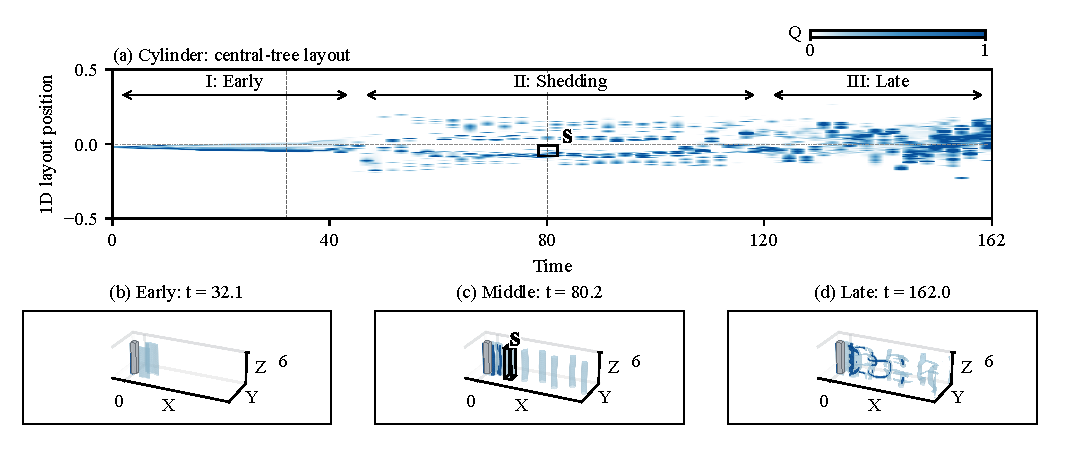
\includegraphics[width=\textwidth]{figures/anchor_cylinder_centered_blue.pdf}
\caption{Cylinder central-tree variant: the full 102-frame map (a) and source $Q$ isosurfaces at three times (b--d), with a common camera and blue scalar scale. $Q=0.2$ is translucent and $Q=1$ marks the core; values above 1 saturate. The outlined component contains extremum S. Map position is not physical $X$; the padded locator and stages I--III are viewing guides, not exact support projections or transition estimates.}
\label{fig:cylinder-centered}
\end{figure*}
The central-tree example is a separate qualitative configuration, excluded from both quantitative tables of the paper. Cylinder comprises 102 volumes ($135\times64\times48$) of the $Q$-criterion with 2\% per-frame persistence. It tests how additional tree guidance changes the map's coordinate interpretation.

The variant in Fig.~\ref{fig:cylinder-centered} uses the same 102 volumes, retained 2\% persistence trees and a 1\% merge allowance. Full-sample tree coordinates $g_i^t\in[-0.5,0.5]$ add $16\,\mathrm{mean}_i(x_i^t-g_i^t)^2$ to the placement objective; reference, geometry, temporal and eccentricity weights are 1, 1, 0.5 and 0.1. True-$X$ targets retain one fixed domain transform. This changes multiple weights and is not a single-factor ablation.

Its fixed tree-compatible order needs a worst-case reference cap of 55.21\%; we explicitly allow 56.21\%, including 1\% slack. Monotone warping of the tree profile through the optimized intervals produces 32768-position rasters. All retained-pair checks yield NMLE$_{max}=0$, within 1\%, including half-pixel position rounding; this conservative order does not exploit budgeted reordering or introduce simulation frames.

Central guidance exposes unfolding but sacrifices anchoring. Frame-balanced mean absolute $X$ error is 21.1\%, 25.5\% and 28.1\% for guidance weights 1, 4 and 16, versus 1.9\% for the Cartesian-reference configuration. This differs from NPE and pooled mean displacement. These outputs are not the Cartesian-reference configurations of the paper's volumetric table. Equal-$X$ features may differ in $Y,Z$; their layout separation does not encode depth.

\FloatBarrier
\section{Complete Results by Method}\label{sec:complete}
This section lists every measured value of the paper, one table per group of measures, with one column per method. Tables~\ref{tab:full-order}, \ref{tab:full-bound-other} and~\ref{tab:full-planar-positions} cover the bound suite, Tables~\ref{tab:full-layout} and~\ref{tab:full-volume} the layout suite. Percentages refer to the canvas (order error, displacement) or to the scalar range (merge error). Every baseline is shown in the mirror stated in Section~\ref{sec:baselines}. A dash marks a method that does not apply: the curves are defined on planar grids only, and OLO yields an order without anchors.

\begin{table*}[t]
\centering\small
\caption{Bound suite: mean order error NROE (top) and worst merge error over frames NMLE (bottom), in percent. $\nu^*$ is the exact-topology bound. AnchorMTM keeps the numerical allowance $\varepsilon_0$ in Exact Mode, which merges saddles tied within $10^{-7}$ of the scalar range; on Cylinder this lowers its order error below the strict $\nu^*$ at a merge error below $10^{-5}$\%.}\label{tab:full-order}
\setlength{\tabcolsep}{4pt}
\begin{tabular}{lr|rrr|rrr|rr}\toprule
 & & \multicolumn{3}{c|}{keep the tree} & \multicolumn{3}{c|}{follow space} & \multicolumn{2}{c}{AnchorMTM}\\
Sequence & $\nu^*$ & OLO & TMTM & ST-MTM & Hilbert & Morton & Projection & $\varepsilon=0$ & $\varepsilon=10\%$\\\midrule
\multicolumn{10}{l}{\emph{Order error NROE (\%)}}\\
Storms & 3.77 & 15.60 & 18.31 & 16.28 & 8.46 & 5.56 & 0 & 3.77 & 1.43\\
Wildfires & 5.80 & 19.06 & 19.65 & 18.72 & 12.60 & 2.40 & 0 & 5.80 & 1.09\\
OLR & 0.89 & 16.27 & 19.31 & 16.59 & 1.60 & 0.91 & 0 & 0.89 & 0.30\\
PM$_{2.5}$ (daily) & 0.97 & 5.17 & 4.44 & 5.21 & 0.97 & 0.27 & 0 & 0.98 & 0.00\\
Ring & 2.66 & 4.23 & 7.18 & 4.47 & 2.61 & 1.12 & 0 & 2.66 & 0.05\\
Tangaroa & 9.24 & 15.44 & 19.50 & 15.80 & -- & -- & 0 & 9.67 & 4.76\\
Cylinder & 12.24 & 18.03 & 26.62 & 17.77 & -- & -- & 0 & 8.01 & 0.01\\\midrule
\multicolumn{10}{l}{\emph{Worst merge error NMLE (\%)}}\\
Storms & & 0 & 0 & 0 & 39.47 & 39.47 & 58.66 & 0 & 8.51\\
Wildfires & & 0 & 0 & 0 & 29.51 & 40.12 & 52.58 & 0 & 8.35\\
OLR & & 0 & 0 & 0 & 24.01 & 24.01 & 33.56 & 0 & 5.15\\
PM$_{2.5}$ (daily) & & 0 & 0 & 0 & 11.42 & 11.42 & 5.62 & 0 & 5.62\\
Ring & & 0 & 0 & 0 & 7.87 & 10.12 & 12.35 & 0 & 9.40\\
Tangaroa & & 0 & 0 & 0 & -- & -- & 31.02 & 0 & 9.97\\
Cylinder & & 0 & 0 & 0 & -- & -- & 14.28 & 0 & 9.71\\\bottomrule
\end{tabular}
\end{table*}

\begin{table*}[t]
\centering\small
\caption{Bound suite: motion error ME (percent of clear approach or separation events shown in the wrong direction or not at all), scale-normalized stress SNS and trustworthiness TW ($k=1$). AnchorMTM uses the default configuration $\Theta_0$. Daily PM$_{2.5}$ contains few clear events and was not used for the motion reading of the paper.}\label{tab:full-bound-other}
\setlength{\tabcolsep}{3.2pt}
\begin{tabular}{l|rrr|rrr|rrr|rrr|rrr}\toprule
 & \multicolumn{3}{c|}{TMTM} & \multicolumn{3}{c|}{ST-MTM} & \multicolumn{3}{c|}{Projection} & \multicolumn{3}{c|}{AnchorMTM, $\varepsilon=0$} & \multicolumn{3}{c}{AnchorMTM, $\varepsilon=10\%$}\\
Sequence & ME & SNS & TW & ME & SNS & TW & ME & SNS & TW & ME & SNS & TW & ME & SNS & TW\\\midrule
Storms & 47.1 & 0.080 & 0.824 & 41.3 & 0.030 & 0.965 & 14.4 & 0.106 & 0.723 & 24.0 & 0.120 & 0.770 & 19.2 & 0.113 & 0.752\\
Wildfires & 39.3 & 0.221 & 0.817 & 35.7 & 0.079 & 0.919 & 33.0 & 0.057 & 0.861 & 34.8 & 0.085 & 0.875 & 34.8 & 0.061 & 0.876\\
OLR & 44.6 & 0.142 & 0.814 & 21.4 & 0.006 & 0.975 & 5.4 & 0.009 & 0.961 & 5.4 & 0.012 & 0.956 & 7.1 & 0.010 & 0.962\\
PM$_{2.5}$ (daily) & 45.3 & 0.051 & 0.760 & 51.6 & 0.026 & 0.922 & 49.5 & 0.052 & 0.725 & 44.2 & 0.065 & 0.751 & 49.5 & 0.052 & 0.727\\
Ring & 64.5 & 0.171 & 0.707 & 34.7 & 0.080 & 0.917 & 12.1 & 0.143 & 0.698 & 31.5 & 0.164 & 0.686 & 11.3 & 0.142 & 0.707\\
Tangaroa & 97.5 & 0.525 & 0.670 & 70.0 & 0.165 & 0.814 & 30.5 & 0.335 & 0.748 & 52.2 & 0.362 & 0.726 & 41.3 & 0.341 & 0.754\\
Cylinder & 67.0 & 0.296 & 0.802 & 46.0 & 0.135 & 0.899 & 19.3 & 0.043 & 0.878 & 33.1 & 0.110 & 0.814 & 19.5 & 0.041 & 0.889\\\bottomrule
\end{tabular}
\end{table*}

\begin{table*}[t]
\centering\small
\caption{Layout suite, planar inputs: the measures of the paper's comparison table rearranged with one column per method. AnchorMTM's budgeted column is Balanced (1, 1, 5 and 10\% on Gaussian, Ring, Wildfires and Storms) and a fixed 5\% on PM$_{2.5}$; its attained worst merge error is 0, 0.982, 4.421, 9.985 and 4.998\%, and Exact has zero merge error. $^\dagger$Published values of the ST-MTM paper on the authors' inputs, not ranked against local values.}\label{tab:full-layout}
\setlength{\tabcolsep}{5pt}
\begin{tabular}{l|rr|rr|rr}\toprule
 & \multicolumn{2}{c|}{follow space} & \multicolumn{2}{c|}{keep the tree} & \multicolumn{2}{c}{AnchorMTM}\\
Input & Hilbert & Morton & TMTM & ST-MTM & Exact & budgeted\\\midrule
\multicolumn{7}{l}{\emph{NPE: mean worst displacement per frame (fraction of the extent) $\downarrow$}}\\
Gaussian & 0.7557 & 0.7359 & 0.1118 & 0.1154 & 0.0089 & 0.0089\\
Ring & 0.5941 & 0.6033 & 0.1756 & 0.2463 & 0.0471 & 0.0395\\
Wildfires & 0.3641 & 0.1560 & 0.2280 & 0.3180 & 0.0131 & 0.0116\\
Storms & 0.3705 & 0.3468 & 0.5753 & 0.4579 & 0.0399 & 0.0140\\
PM$_{2.5}$ (hourly) & 0.8090 & 0.8823 & 0.5241 & 0.5577 & 0.1390 & 0.0468\\\midrule
\multicolumn{7}{l}{\emph{SNS: scale-normalized stress $\downarrow$}}\\
Gaussian & 0.1117 & 0.0393 & 0.2500$^\dagger$ & 0.0600$^\dagger$ & 0.0353 & 0.0353\\
Ring & 0.1252 & 0.1489 & 0.2800$^\dagger$ & 0.2100$^\dagger$ & 0.1485 & 0.1334\\
Wildfires & 0.1883 & 0.1304 & 0.4400$^\dagger$ & 0.2400$^\dagger$ & 0.0426 & 0.0447\\
Storms & 0.1290 & 0.1180 & 0.3400$^\dagger$ & 0.2100$^\dagger$ & 0.0790 & 0.0743\\
PM$_{2.5}$ (hourly) & 0.2386 & 0.1760 & 0.3018 & 0.1897 & 0.1964 & 0.1636\\\midrule
\multicolumn{7}{l}{\emph{TW: trustworthiness $\uparrow$}}\\
Gaussian & 0.6719 & 0.8333 & 0.7700$^\dagger$ & 1.0000$^\dagger$ & 0.9323 & 0.9323\\
Ring & 0.9048 & 0.7619 & 0.6800$^\dagger$ & 0.8800$^\dagger$ & 0.8571 & 0.8571\\
Wildfires & 0.8303 & 0.8758 & 0.8800$^\dagger$ & 0.9100$^\dagger$ & 0.9136 & 0.8989\\
Storms & 0.7403 & 0.7251 & 0.7100$^\dagger$ & 0.9400$^\dagger$ & 0.8463 & 0.8766\\
PM$_{2.5}$ (hourly) & 0.8887 & 0.8277 & 0.7781 & 0.8224 & 0.7884 & 0.7657\\\bottomrule
\end{tabular}
\end{table*}

\begin{table*}[t]
\centering\small
\caption{Bound suite, planar sequences, default configuration: the positions of Fig.~\ref{fig:supp-positions}. Mean displacement over all features and NPE in percent of the canvas, worst merge error in percent of the scalar range. Native maps are rescaled to the canvas and shown in their more favourable mirror; their per-frame order reproduces the stored NROE exactly.}\label{tab:full-planar-positions}
\setlength{\tabcolsep}{4.2pt}
\begin{tabular}{ll|rr|rrr}\toprule
 & & \multicolumn{2}{c|}{keep the tree} & \multicolumn{3}{c}{AnchorMTM, budget $\varepsilon$}\\
Sequence & Measure & TMTM & ST-MTM & 0 & 5\% & 20\%\\\midrule
Wildfires & mean displacement & 19.62 & 22.23 & 3.24 & 1.44 & 0.78\\
 & NPE & 46.80 & 38.53 & 6.93 & 2.94 & 1.19\\
 & worst merge error & 0 & 0 & 0 & 4.99 & 19.56\\
OLR & mean displacement & 29.65 & 26.72 & 1.00 & 0.77 & 0.62\\
 & NPE & 50.92 & 47.04 & 1.72 & 1.22 & 0.88\\
 & worst merge error & 0 & 0 & 0 & 2.43 & 19.77\\
PM$_{2.5}$ (daily) & mean displacement & 17.14 & 24.56 & 1.87 & 0.75 & 0.75\\
 & NPE & 24.08 & 33.11 & 1.85 & 0.70 & 0.69\\
 & worst merge error & 0 & 0 & 0 & 4.67 & 5.62\\
Ring & mean displacement & 26.84 & 23.83 & 2.44 & 1.20 & 0.62\\
 & NPE & 43.74 & 41.58 & 3.40 & 1.46 & 0.67\\
 & worst merge error & 0 & 0 & 0 & 4.97 & 12.35\\\bottomrule
\end{tabular}
\end{table*}

\begin{table*}[t]
\centering\small
\caption{Layout suite, volumes. Top: stored configurations with the $+x$ reference (the paper's volumetric table; Balanced uses 1\% on Cylinder and 33.33\% on Tangaroa). Bottom: default configuration with the references of Fig.~\ref{fig:supp-positions}; mean displacement and NPE in percent of the canvas, worst merge error in percent of the scalar range. Native maps are rescaled to the canvas and shown in their more favourable mirror.}\label{tab:full-volume}
\setlength{\tabcolsep}{4.2pt}
\begin{tabular}{ll|rr|rrrrr}\toprule
\multicolumn{9}{l}{\emph{Stored configurations, $+x$ reference}}\\
 & & \multicolumn{2}{c|}{} & \multicolumn{5}{c}{AnchorMTM}\\
Volume & Measure & TMTM & & Exact & Balanced & & & \\\midrule
Cylinder & SNS $\downarrow$ / TW $\uparrow$ / NPE $\downarrow$ & 0.2956 / 0.8017 / 0.4769 & & 0.1226 / 0.8010 / 0.1773 & 0.0329 / 0.9117 / 0.0458 & & & \\
Tangaroa & SNS $\downarrow$ / TW $\uparrow$ / NPE $\downarrow$ & 0.5255 / 0.6701 / 0.3866 & & 0.1204 / 0.8213 / 0.1285 & 0.1124 / 0.8408 / 0.0653 & & & \\\midrule
\multicolumn{9}{l}{\emph{Default configuration}}\\
 & & \multicolumn{2}{c|}{keep the tree} & \multicolumn{5}{c}{AnchorMTM, budget $\varepsilon$}\\
Volume & Measure & TMTM & ST-MTM & 0 & 2\% & 5\% & 10\% & 20\%\\\midrule
Tangaroa & mean displacement & 8.81 & 13.44 & 5.01 & 4.55 & 3.99 & 3.02 & 1.27\\
 & NPE & 30.63 & 34.18 & 11.18 & 10.03 & 8.91 & 6.15 & 1.87\\
 & worst merge error & 0 & 0 & 0 & 2.00 & 4.98 & 9.97 & 19.94\\
Cylinder & mean displacement & 26.62 & 24.31 & 3.76 & 0.64 & 0.56 & 0.54 & 0.54\\
 & NPE & 47.69 & 51.60 & 9.18 & 1.28 & 1.19 & 1.16 & 1.16\\
 & worst merge error & 0 & 0 & 0.00 & 1.67 & 4.79 & 9.71 & 14.28\\\bottomrule
\end{tabular}
\end{table*}


\FloatBarrier
\bibliographystyle{abbrv-doi-narrow}
\bibliography{refs}
\end{document}
